\documentclass[11pt,a4paper]{article}
\usepackage[utf8]{inputenc}
\usepackage[german]{babel}
\usepackage{amsmath}
\usepackage{amsfonts}
\usepackage{amssymb}
\usepackage{float}
\usepackage{graphicx}
\usepackage{mwe}
\usepackage{changepage}
\usepackage[margin=100pt]{geometry}
\usepackage{tabularx}
\usepackage{color, colortbl}
\usepackage{multirow}
\usepackage{lmodern, textcomp}
\usepackage{fancyhdr}
\usepackage{lscape}
\usepackage{verbatim}
\usepackage{tikz}
\usepackage[usestackEOL]{stackengine}
\author{Georg Felber, Markus Mondl, Florian Ritter, Luca Wenzl}

\newenvironment{indentE}{\begin{adjustwidth}{0.5cm}{}}{\end{adjustwidth}}

\usepackage{xparse}

\ExplSyntaxOn
\NewDocumentCommand{\NewWeirdCommand}{mm}
{% #1 = command to define, #2 = replacement text
	\cs_new:Npn #1 ##1
	{
		\tl_set:Nn \l__simon_args_tl { ##1 }
		#2
	}
}
\NewDocumentCommand{\Arg}{m}
{
	\tl_item:Nn \l__simon_args_tl { #1 }
}

\tl_new:N \l__simon_parse_args_tl
\ExplSyntaxOff

\NewWeirdCommand{\UseCase}{\\\\
	\begin{table}[H]
		\begin{center}
			\begin{tabularx}{\linewidth}{|l|X|}
				\hline
				\multicolumn{2}{|c|}{\multirow{2}{*}{\large\textbf{\Arg{2}}}}\\
				\multicolumn{2}{|c|}{} \\
				\hline
				\multicolumn{2}{|l|}{\multirow{2}{*}{\large\textbf{UseCase}}}\\
				\multicolumn{2}{|l|}{} \\
				\hline\textbf{Art}&
				\Arg{1}\\
				%\rowcolor{LBlue}
				\hline\textbf{Beschreibung}&
				\Arg{4}\\
				\hline\textbf{Auslöser}&
				\Arg{5}\\
				%\rowcolor{LBlue} 
				\hline\textbf{Ergebnis}&
				\Arg{6}\\
				\hline\textbf{Akteure}&
				\Arg{7}\\
				%\rowcolor{LBlue}
				\hline\textbf{Informationen}&
				\Arg{8}\\
				\hline\textbf{Vorbedingungen}&
				\Arg{9}\\
				%\rowcolor{LBlue}
				\hline\textbf{Nachbedingung}&
				\Arg{10}\\
				\hline\textbf{Nutzen}&
				\Arg{11}\\
				%\rowcolor{LBlue}
				\hline\textbf{Aufwand}&
				\Arg{12}\\
				\hline\textbf{Priorität}& 
				\Arg{13}\\
				\hline
			\end{tabularx}
		\end{center}
	\end{table}
	\newpage
}

\pagestyle{fancy}
\lhead{Pflichtenheft Phobos-Wireless}
\rhead{Team Phobos}
\lfoot{\hline \mbox{}\\ V1}
\cfoot{}
\rfoot{\hline \mbox{} \\ \thepage}

\title{Pflichtenheft Phobos-Wireless}
\begin{document}
	\maketitle
	\thispagestyle{empty}
	\tikz[remember picture,overlay]
	\node[anchor=north east,inner sep=10pt] at (current page.north east)
	{
\includegraphics[height=3cm]{pictures/logo/logo.jpg}};
	\mbox{}\\
	\begin{table}[H]
		\begin{center}
			\begin{tabularx} {\linewidth}{|l|c|c|l|c|X|}
				\hline
				\textbf{V} & 
				\textbf{Autor} &
				\textbf{QS} & 
				\textbf{Datum} & 
				\textbf{Status} & 
				\textbf{Kommentar}\\\hline
				0.1 & gfelber & fritter & 22.3.2019 & Entwurf & Zielbestimmungen hinzugefügt\\
				\hline
				0.2 & gfelber & fritter & 23.3.2019 & Überarbeitet & Produktfunktionen hinzugefügt\\
				\hline
				0.2 & gfelber & fritter & 24.3.2019 & Überarbeitet & Produktleistungen hinzugefügt\\
				\hline
				0.3 & gfelber & fritter & 25.3.2019 &Überarbeitet & Qualitätsbestimmungen \& Sonstiges hinzugefügt\\
				\hline
				0.4 & mmondl & fritter & 25.3.2019 & Überarbeitet & Produkteinsatz hinzugefügt\\
				\hline
				0.5 & mmondl & fritter & 26.3.2019 & Überarbeitet & Vertragsgegenstand hinzugefügt\\
				\hline
				0.6 & gfelber & fritter & 26.3.2019 & Überarbeitet & Sonstiges hinzugefügt\\
				\hline
				1 & gfelber & ZAKS & 28.3.2019 & Überarbeitet & Sonstiges hinzugefügt\\
				\hline
			\end{tabularx}
		\end{center}
	\end{table}
	\newpage
	\tableofcontents
	\newpage
	\section{Einleitung}
Im Rahmen des Projekts wird das Projektteam eine Desktop-Applikation welche auf der Projektwebseite erhältlich ist, eine Mobile Version die für 5€ auf Google Play Store verfügbar ist, als auch die zuvor erwähnte Projektwebseite mit der das fertige Produkt vorgestellt wird, entwickelt. Die Webseite wird auch einen Shop enthalten mit welchem der Benutzer die Desktop-Applikation kaufen und downloaden kann. Die Benutzung der Webseite oder genauer gesagt dem Shop ist für jeden Besucher offen und benötigt daher keine Erstellung eines Benutzers.
\\\\
Genau wie bei der Verwendung der Webseite ist auch bei der Desktop-Applikation bzw. der Mobilen Version kein Benutzerprofil nötig. Bei beiden Applikationen muss der Benutzer zuerst den Empfänger auswählen und eine Verbindung mit diesem aufbauen. Nach dem erfolgreichen Verbindungsaufbau kann man mit nur einem Knopfdruck die zu versendende Datei auswählen und absenden.  %Markus
	\newpage
	\section{Zielbestimmungen}
Nach Abschluss des Projekts soll es dem Benutzer möglich sein, mit Hilfe der beiden Komponenten kabellos und ohne Internetverbindung jede belibige Datei zwischen zwei Geräten zu übertragen. Hierbei ist zu beachten, dass der Datentransfer nur vonstatten gehen kann wenn beide Komponenten installiert sind.
Durch die Verwendung des Produkts soll der Benutzer immer und überall die Möglichkeit haben schnell und einfach seine Daten mit einem anderen Gerät zu sharen. Dies führt zu einer  Zeitersparnis für den Benutzer.\\
 %Georg
	\newpage
	\section{Produkteinsatz}
Grundsätzlich ist das Produkt für Jugendliche oder berufstätige Personen, welche nicht in der Lage sind einen Datentransfer immer mit Internet oder Kabel durchzuführen, gedacht. Durch den Einsatz des fertigen Produkts erspart sich der Benutzer nicht nur einiges an Zeit sondern er kann es auch jederzeit und ohne einer Internetverbindung benutzen.\\ %Markus
	\newpage
	\section{Produktumgebung}
Dieser Bereich weißt auf Umgebungsinformationen des Fertigproduktes hin und beschreibt diese kompakt.
\subsection{Software}
Voraussetzungen für die Nutzung des fertigen Produktes sind die Betriebssysteme Windows 7 oder höher, Android 4.3 oder höher, oder MacOS, sowie iOS. Fertiggestellt wird das Produkt über die inkludierte Webseite vorhanden sein. Zudem wird eine Mobilversion im Google-PlayStore veröffentlicht. Hyperreferenzen zu den einzelnen Unterprodukten sind auf der Webseite eingebunden.
\subsection{Hardware}
Um dem Anwender eine angenehme Nutzererfahrung zu bieten, ist es empfohlen ein System zu nutzen, welches einen Prozessor von mindestens einem GHz auf einem Kern unterstützt. Weiters sind RAM-Bausteine zusammenfassend bei mindestens 1 GiB und einen Bildschirm im Mindestformat WVGA zu benutzen, da die Applikation sonst nicht ordnungsgemäß arbeiten kann. Der Speicher sollte ein Minimum von 20 MB freiem Speicherplatz auf jedem Gerät nicht unterschreiten. Die Nutzung von Hintergrundapplikationen, welche das System zusätzlich belasten, ist nicht eingerechnet.
\subsection{Produkt-Schnittstelle}
Um einen einwandfreien Datentransfer zu ermöglichen ist eine BlueTooth Schnittstelle per Gerät vorausgesetzt. Wenn dies nicht gegeben ist, funktionieren die Anwendungen nicht wie gefordert. %Florian
	\newpage
	\section{Produktfunktionen}
Es werden die Funktionen anhand von verschieden Kriterien beschrieben. Diese können im genaueren aus der unteren Tabelle entnommen werden.
\UseCase{
	{Der Bereich, unter welchen die Funktionen fällt}
	{Der Name und die ID der Funktion}
	{Die Art, unter welche die Funktion in dessen Umsetzung fallen wird}
	{Eine kurze Beschreibung der Funktion.}
	{Der Grund für die Existenz der Funktion im Produkt.}
	{Das Ergebnis, welche die Funktion erfüllen soll.}
	{Die verschiedenen Teilnehmer, welche von dieser Funktion betroffen sind.}
	{Die ein- und ausgehenden Informationen welche in Zusammenhang mit dieser Funktion stehen.}
	{Die Bedingungen, welche von dem Eintreffen der Funktion herrschen.}
	{Die Bedingungen, welche nach dem Eintreffen der Funktion herrschen.}
	{Der Nutzen der Funktion: gering, mittel, hoch}
	{Der Aufwand der Funktion: gering, mittel, hoch}
	{Die Priorität der Funktion: Must Have, Should Have, Nice to Have}
}
\subsection{Desktop-Version}
Es werden die Funktionen beschrieben, welche die Desktop-Version des Produktes erfüllen soll. Diese werden grundsätzliche in Frontend und Backend unterteilt.
\subsubsection{Backend erstellen}
Das Backend umfasst alle Funktionen, welche vom Benutzer nicht gesehen werden können. Diese bearbeitet den Datentransfer, Datenaufbereitung und die Datensicherheit.
\paragraph{Aktivitätsdiagramm Backend}\mbox{}\\
\begin{figure}[H]
	\centering
	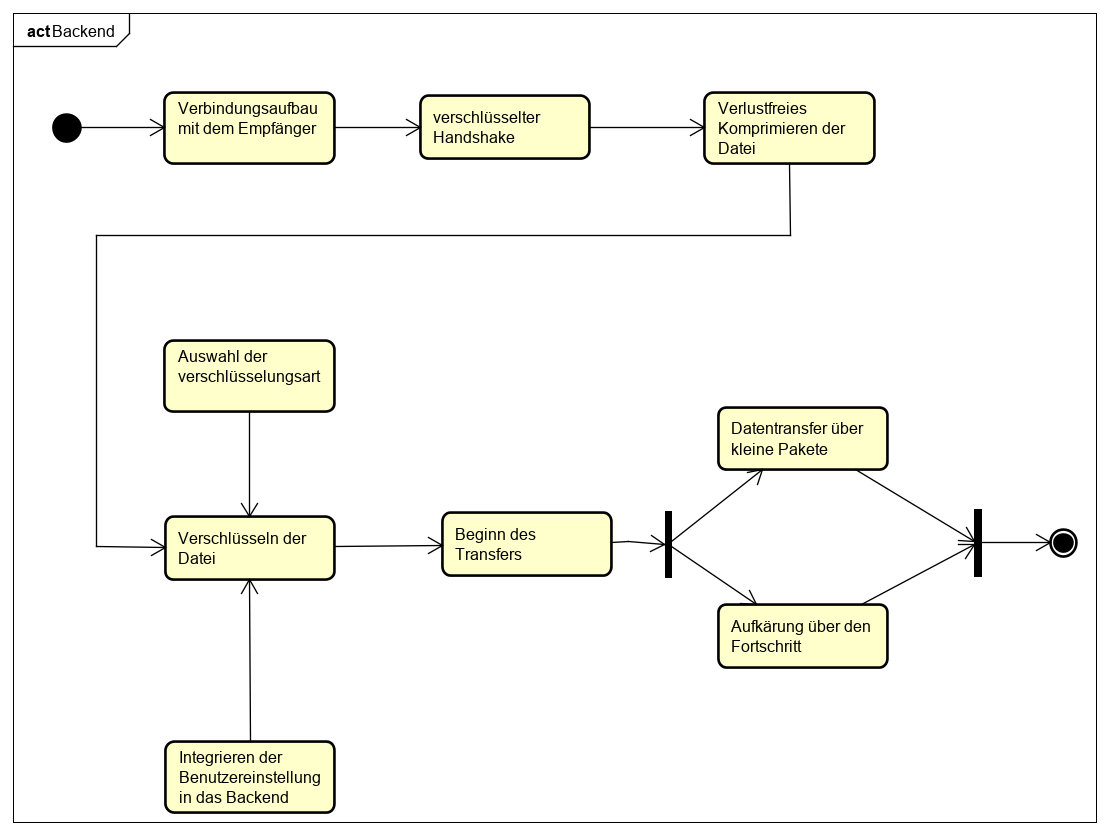
\includegraphics[width= 0.9\linewidth]{diagramms/activity/Backend.png}
	\caption{Aktivitätsdiagramm Backend}
\end{figure}
\newpage
\begin{indentE}\mbox{}
	\paragraph{/LF1110/ Verbindung aufbauen}\mbox{}\\
	Es wird die Verbindung mit dem ausgewählten Empfänger aufgebaut. Dieser Verbindungsaufbau besteht aus einem verschlüsselten Handshake, mit welchem die Systemdaten des Empfängers und Senders ausgetauscht werden. Wenn Empfänger und Sender den selben Verschlüsselungsschlüssel gewählt haben, ist der Handshake erfolgreich und der Transfer kann beginnen.
	\UseCase{
		{Desktop Backend}
		{/LF1110/ Verbindung aufbauen}
		{Backend}
		{Es wird die Verbindung mit dem Empfänger als Sender aufgebaut.}
		{Es muss eine Verbindung zwischen Empfänger und Sender für den Datentransfer herrschen}
		{Der Empfänger kann sich mit einem Empfänger der Wahl verbinden.}
		{Empfänger, Sender}
		{Sender, Namen }
		{Der Sender kann sich nicht mit dem Empfänger verbinden.}
		{Der Sender kann sich mit dem Empfänger verbinden.}
		{hoch}
		{mittel}
		{Must Have}
	}
	\paragraph{/LF1120/ Daten transferieren}\mbox{}\\
	Die Daten werden in kleinen Paketen versandt, um die Datensicherheit zu garantieren. Dabei haben diese eine einheitliche Größe und es werden unterschiedliche viele je nach Datengröße versandt. Dabei sollen der Empfänger und der Sender um den Fortschritt der Übertragung aufgeklärt werden.
	\UseCase{
		{Desktop Backend}
		{/LF1120/ Daten transferieren}
		{Backend}
		{Die Daten sollen vom Sender zum Empfänger transferiert werden. Diese soll dabei möglichst verlustlos gesendet werden.}
		{Der Daten müssen an den Empfänger gebracht werden.}
		{Die Daten des Sender kommen beim Empfänger an.}
		{Empfänger, Sender}
		{Datei(Name, Größe, Inhalt), Fortschritt(aus index und Anzahl Pakete), Sender, Empfänger}
		{Die Daten können dem Empfänger nicht vom Sender geschickt werden.}
		{Die Daten werden vom Sender zum Empfänger verlustlos gesendet.}
		{hoch}
		{gering}
		{Must Have}
	}
	\paragraph{/LF1130/ Daten komprimieren}\mbox{}\\
	Die Daten werden vor dem Versand verlustlos komprimiert, um die Datenmenge zu verkleinern. Die dabei gewählt Komprimierungsart, darf vom Auftragnehmer ausgewählt werden.
	\UseCase{
		{Desktop Backend}
		{/LF1130/ Daten komprimieren}
		{Backend}
		{Die Daten sollen vor dem Transfer verlustlos komprimiert werden, um die Übertragungsdauer zu verringern}
		{Der Datentransfer soll kürzer dauern.}
		{Der Datentransfer dauert in den meisten Fällen kürzer.}
		{Sender, Empfänger}
		{Daten}
		{Die Datenübertragung dauert länger.}
		{Die Datenübertragung dauert kürzer.}
		{mittel}
		{mittel}
		{Should Have}
	}
	\paragraph{/LF1140/ Datentransfer verschlüsseln}\mbox{}\\
	Der Datentransfer wird mit einem Verschlüsselungsschlüssel nach dem AES256 Standard verschlüsselt, um die Datensicherheit zu erhöhen. Diese wird dann vom Empfänger wieder entschlüsselt. Die dafür benutzte Verschlüsselungsart, kann vom Auftraggeber ausgewählt werden.
	\UseCase{
		{Desktop Backend}
		{/LF1140/ Datentransfer verschlüsseln}
		{Backend}
		{Der Datentransfer soll für eine höhere Sicherheit durch einen Schlüssel verschlüsselt werden.}
		{Der Datentransfer soll verschlüsselt stattfinden, damit die originalen Daten nicht von Dritten ausgelesen werden können.}
		{Der Datentransfer erfüllt den Standard AES256.}
		{Empfänger, Sender, Dritte}
		{Daten, Schlüssel}
		{Die originalen Daten können von Dritten ausgelesen werden}
		{Die originalen Daten sind während dem Transfer verschlüsselt}
		{mittel}
		{mittel}
		{Must Have}
	}
	\paragraph{/LF1150/ Benutzereinstellungen integrieren}\mbox{}\\
	Die vom Benutzer ausgewählten Benutzereinstellungen müssen in das Backend integrierte werden, um den Nutzen aus diesen Werten zu ziehen.
	\UseCase{
		{Desktop Backend}
		{/LF1150/ Benutzereinstellungen integrieren}
		{Backend}
		{Die Benutzereinstellungen sollen integriert werden.}
		{Die ausgewählten Benutzereinstellungen sollen in das Backend integriert werden.}
		{Die Einstellungen des Benutzer haben eine Auswirkung auf das Backend.}
		{Sender, Empfänger}
		{gewünschte Systemname, Verschlüsselung (Ja/Nein), Standardschlüssel, Speicherort}
		{Der Benutzer muss die meisten Daten bei jeder Übertragung neu einstellen, wodurch diese länger dauert}
		{Der Übertragung ist anpassbar, wodurch diese verschnellert werden kann. }
		{mittel}
		{gering}
		{Should Have}
	}
\end{indentE}
\subsubsection{Frontend erstellen}
Zu dem Frontend des Produktes gehören alle Elemente, auf welche der Benutzer Einsicht hat und mit denen er interagieren kann. Diese sind besonders für die Benutzbarkeit des Produkt wichtig, da diese die wichtigste Produktqualität ist.
\paragraph{Aktivitätsdiagramm Frontend}\mbox{}\\
\begin{figure}[H]
	\centering
	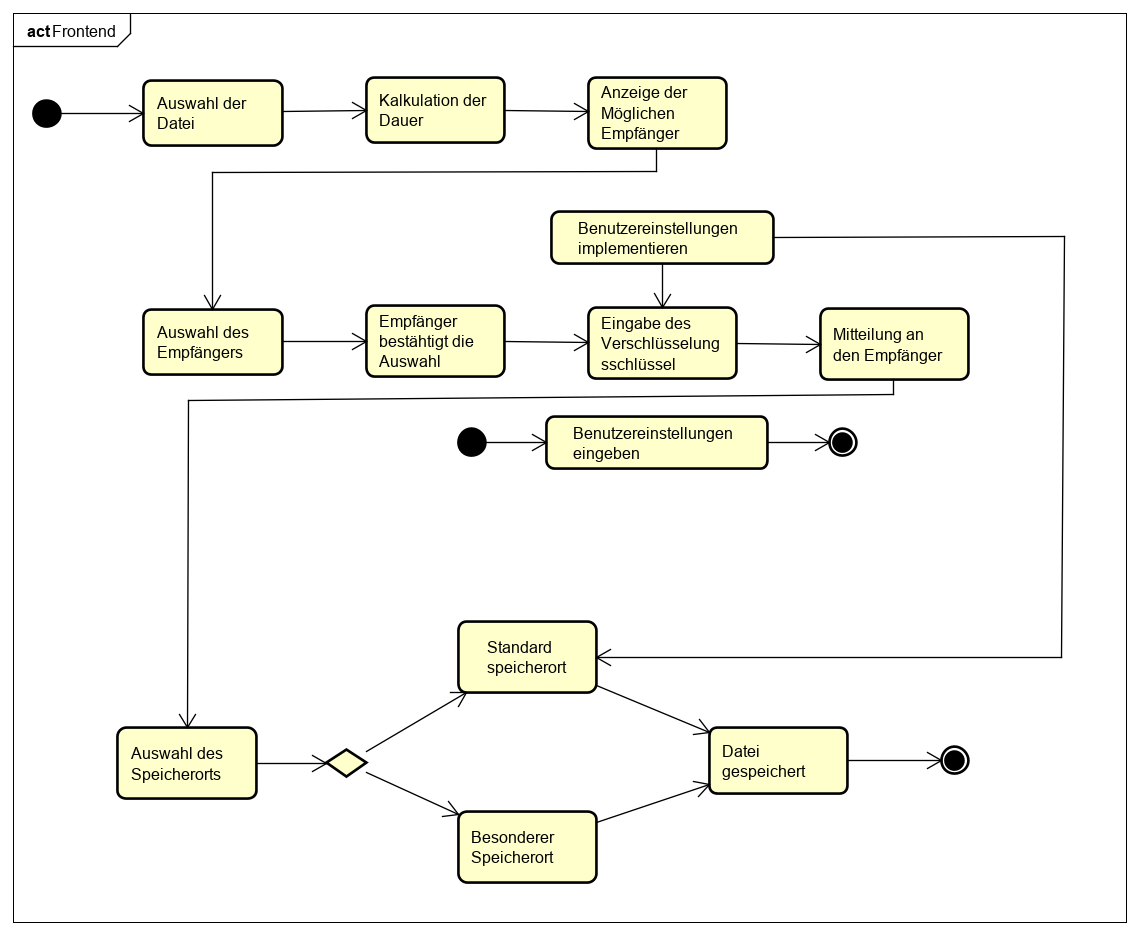
\includegraphics[width= 0.9\linewidth]{diagramms/activity/Frontend.png}
	\caption{Aktivitätsdiagramm Frontend}
\end{figure}
\newpage
\begin{indentE}\mbox{}
	\paragraph{/LF1210/ Datei auswählen}\mbox{}\\
	Der Benutzer wählt eine Datei aus, welche er verschicken möchte. Hierbei soll eine voreilige Kalkulation durchgeführt werden, welche die Dauer der Übertragung schätzt.
	\UseCase{
		{Desktop Frontend}
		{/LF1210/ Datei auswählen}
		{Frontend}
		{Ein wird die zu versendende Datei ausgewählt.}
		{Es muss die Datei, welche versendet werden soll, ausgewählt werden}
		{Es kann die Datei gesendet werden}
		{Sender}
		{Datei(Name, Größe, Inhalt)}
		{Es kann keine Datei ausgewählt werden}
		{Es kann eine zu versendende Datei ausgewählt werden}
		{hoch}
		{mittel}
		{Must Have}
	}
	\paragraph{/LF1220/ Empfänger auswählen}\mbox{}\\
	Es werden dem Benutzer die möglichen Empfänger angezeigt und ausgwählt oder er kann den Namen des Empfängers eingeben, um den Empfänger zu bestimmen. Dieser muss die Verbindung bestätigen.
	\UseCase{
		{Desktop Frontend}
		{/LF1220/ Empfänger auswählen}
		{Frontend}
		{Der Sender wählt anhand des Namens den Empfänger aus, mit dem der Datentransfer stattfinden soll.}
		{Es muss der Empfänger ausgewählt werden.}
		{Die Verbindung kann aufgebaut werden}
		{Sender, Empfänger}
		{Sendername, Empfängername}
		{Es kann kein Empfänger ausgewählt werden.}
		{Es kann anhand des Namens der Empfänger der Datei ausgewählt werden.}
		{hoch}
		{mittel}
		{Must Have}
	}
	\paragraph{/LF1230/ Verschlüsselungsschlüssel eingeben}\mbox{}\\
	Wenn kein Standard-Schlüssel ausgewählt ist, muss der Sender diesen bevor dem Verbindungsaufbau eingeben. Dieser muss dann dem Empfänger mitgeteilt werden und dieser muss den selben auch eingeben, um den Datentransfer zu ermöglichen.
	\UseCase{
		{Desktop Frontend}
		{/LF1230/ Verschlüsselungsschlüssel eingeben}
		{Frontend}
		{Es müssen Empfänger und Sender einen Schlüssel eingeben, die übereinstimmen, um den Datentransfer zu beginnen.}
		{Der Datentransfer muss mit einem Schlüssel verschlüsselt werden.}
		{Der Datentransfer kann verschlüsselt werden}
		{Sender, Empfänger}
		{Schlüssel}
		{Die Daten können nicht mit einem Schlüssel verschlüsselt werden}
		{Die Daten können mit einem frei wählbaren Schlüssel verschlüsselt werden}
		{hoch}
		{mittel}
		{Must Have}
	}
	\paragraph{/LF1240/ Datei speichern}\mbox{}\\
	Der Empfänger soll nach dem empfangen der Datei auswählen können, ob diese im Standard-Speicherort gespeichert wird, oder in einem besonderen. Wenn der Besondere ausgewählt worden ist, soll ihm ein Benutzerinterface gezeigt werden, indem er den Speicherort auswählen.
	\UseCase{
		{Desktop Frontend}
		{/LF1240/ Datei speichern}
		{Frontend}
		{Der Empfänger soll den Speicherort des bekommenen Datei auswählen können.}
		{Die Datei muss irgendwo gespeichert werden}
		{Der Speicherort der Datei kann ausgewählt werden}
		{Empfänger}
		{Datei(Name, Größe, Inhalt), Speicherort}
		{Die Datei wird entweder immer am selben Ort, oder nicht gespeichert}
		{Der Speicherort kann frei gewählt werden}
		{mittel}
		{gering}
		{Must Have}
	}
	\paragraph{/LF1250/ Benutzereinstellungen hinzufügen}\mbox{}\\
	Der Benutzer kann einige Fix-Einstellungen auf seinem Produkt tätigen. Darunter zählt die Möglichkeit, den Namen zu ändern, welcher den restlichen Nutzern angezeigt wird, die Verschlüsselung zu aktivieren oder deaktivieren, einen Standardschlüssel auszuwählen und einen Standard-Speicherort auszuwählen. Dabei sollen die eingegebenen Daten auf ihre Korrektheit überprüft werden.
	\UseCase{
		{Desktop Frontend}
		{/LF1250/ Benutzereinstellungen hinzufügen}
		{Frontend}
		{Der Benutzer kann verschiedenen Einstellungen tätigen, mit welche er die Datenübertragung beeinflussen kann.}
		{Die Einstellungen müssen auf einem Interface getätigt werden}
		{Die Einstellungen können getätigt werden}
		{Empfänger, Sender}
		{gewünschter Systemname, Verschlüsselung(Ja/Nein), Standardschlüssel, Standard-Speicherort}
		{Das Produkt kann nicht angepasst werden.}
		{Es können Einstellungen getroffen werden, welche das Produkt beeinflussen.}
		{mittel}
		{mittel}
		{Should Have}
	}
	\paragraph{/LF1260/ Desktopinterface designen}\mbox{}\\
	Es muss ein Interface für den Desktop entworfen werden. Dazu gehören Mockups und Prototypen. Diese müssen vor deren Implementierung vom Auftraggeber bestätigt werden.
	\UseCase{
		{Desktop Frontend}
		{/LF1260/ Desktopinterface designen}
		{Frontend}
		{Es müssen Mockups für die Desktopinterfaces erstellt werden. Diese diene als Vorlage für die Interfaces.}
		{Für einen schnellere und besser Implementierung sollen Mockups als Vorlage dienen.}
		{Die Implementierung ist einfacher, schneller und besser.}
		{Auftraggeber, Auftragnehmer}
		{}
		{Das Interface wird ohne Vorlage erstellt.}
		{Das Interface kann nach einer vom Auftraggeber bestätigten Vorlage erstellt werden.}
		{mittel}
		{gering}
		{Should Have}
	}
	\paragraph{/LF1270/ Desktopinterace implementieren}\mbox{}\\
	Das Desktopinterface muss nach der Bestätigung des Auftraggeber implementiert werden. 
	\UseCase{
		{Desktop Frontend}
		{/LF1270/}
		{Frontend}
		{Das Desktopinterface muss durch die Mockups realisiert werden.}
		{Der Benutzer hat keine Möglichkeit mit dem System zu integrieren}
		{Der Benutzer kann mit dem System interagieren und dadurch dessen Funktionen benutzen.}
		{Benutzer}
		{sämtliche Nutzereingaben}
		{Der Benutzer kann mit dem System nicht interagieren}
		{Der Benutzer ist in der Lage mit dem System zu interagieren}
		{hoch}
		{hoch}
		{Must-Have}
	}
	\paragraph{/LF1280/ Frontend und Backend verbinden}\mbox{}\\
	Es muss eine Verbindung zwischen dem Frontend und Backend erstellt werden, welche die Aufforderungen verarbeitet und zum Backend weiterleitet. Diese Verbindung, soll dem Benutzer entweder mitteilen, wie lange die Verarbeitung noch dauert oder bei kürzeren das wiederholte Aufrufen von Aufforderungen verhindern.
	\UseCase{
		{Desktop Frontend}
		{/LF1280/ Frontend und Backend verbinden}
		{Frontend}
		{Das Frontend muss mit dem Backend verbunden werden, um die Nutzereingaben an das Backend weiterzuleiten. Außerdem soll es Daten ans Frontend schicken, welche über momentane Prozess aufklärt.}
		{Die Daten müssen vom Frontend ans Backend und umgekehrt geschickt werden}
		{Das Frontend kann mit dem Backend und umgekehrt kommunizieren.}
		{Benutzer}
		{sämtliche Nutzereingaben und verwertete Daten}
		{Die Nutzerdaten können nicht an das Backend und die verwerteten Daten nicht ans Frontend geschickt werden.}
		{Daten können zwischen Frontend und Backend ausgetauscht werden.}
		{hoch}
		{mittel}
		{Must-Have}
	}
\end{indentE}
\subsection{App}
Es werden die Funktionen beschrieben, welche die App-Version des Produktes erfüllen soll. Diese werden grundsätzliche in Frontend und Backend unterteilt.
\subsubsection{Backend erstellen}
Das Backend umfasst alle Funktionen, welche vom Benutzer nicht gesehen werden können. Diese bearbeitet den Datentransfer, Datenaufbereitung und die Datensicherheit.

\paragraph{Aktivitätsdiagramm Backend}\mbox{}\\
\begin{figure}[H]
	\centering
	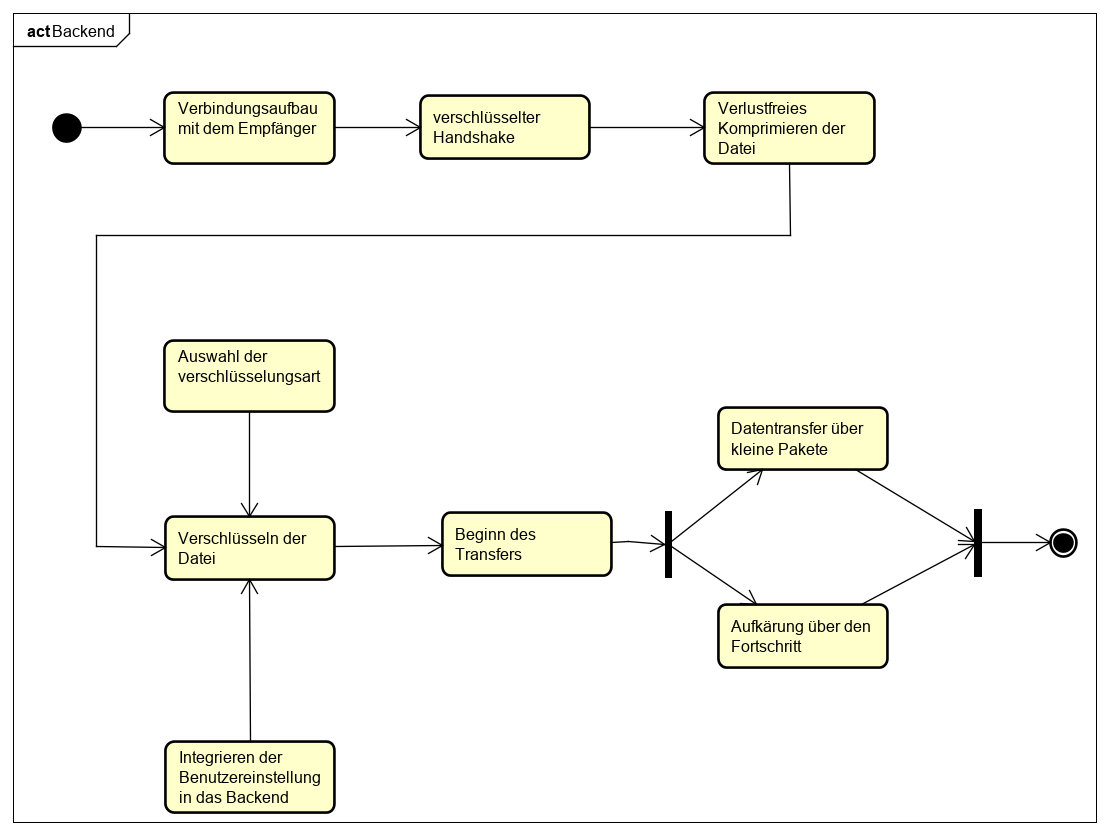
\includegraphics[width= 0.9\linewidth]{diagramms/activity/Backend.png}
	\caption{Aktivitätsdiagramm Backend}
\end{figure}
\newpage
\begin{indentE}\mbox{}
	\paragraph{/LF2110/ Verbindung aufbauen}\mbox{}\\
	Es wird die Verbindung mit dem ausgewählten Empfänger aufgebaut. Dieser Verbindungsaufbau besteht aus einem verschlüsselten Handshake, mit welchem die Systemdaten des Empfängers und Senders ausgetauscht werden. Wenn Empfänger und Sender den selben Verschlüsselungsschlüssel gewählt haben, ist der Handshake erfolgreich und der Transfer kann beginnen.
	\UseCase{
		{App Backend}
		{/LF2110/ Verbindung aufbauen}
		{Backend}
		{Es wird die Verbindung mit dem Empfänger als Sender aufgebaut.}
		{Es muss eine Verbindung zwischen Empfänger und Sender für den Datentransfer herrschen}
		{Der Empfänger kann sich mit einem Empfänger der Wahl verbinden.}
		{Empfänger, Sender}
		{Sender, Namen }
		{Der Sender kann sich nicht mit dem Empfänger verbinden.}
		{Der Sender kann sich mit dem Empfänger verbinden.}
		{hoch}
		{mittel}
		{Should Have}
	}
	\paragraph{/LF2120/ Daten transferieren}\mbox{}\\
	Die Daten werden in kleinen Paketen versandt, um die Datensicherheit zu garantieren. Dabei haben diese eine einheitliche Größe und es werden unterschiedliche viele je nach Datengröße versandt. Dabei sollen der Empfänger und der Sender um den Fortschritt der Übertragung aufgeklärt werden.
	\UseCase{
		{App Backend}
		{/LF2120/ Daten transferieren}
		{Backend}
		{Die Daten sollen vom Sender zum Empfänger transferiert werden. Diese soll dabei möglichst verlustlos gesendet werden.}
		{Der Daten müssen an den Empfänger gebracht werden.}
		{Die Daten des Sender kommen beim Empfänger an.}
		{Empfänger, Sender}
		{Datei(Name, Größe, Inhalt), Fortschritt(aus index und Anzahl Pakete), Sender, Empfänger}
		{Die Daten können dem Empfänger nicht vom Sender geschickt werden.}
		{Die Daten werden vom Sender zum Empfänger verlustlos gesendet.}
		{hoch}
		{gering}
		{Should Have}
	}
	\paragraph{/LF2130/ Daten komprimieren}\mbox{}\\
	Die Daten werden vor dem Versand verlustlos komprimiert, um die Datenmenge zu verkleinern. Die dabei gewählt Komprimierungsart, darf vom Auftragnehmer ausgewählt werden.
	\UseCase{
		{App Backend}
		{/LF2130/ Daten komprimieren}
		{Backend}
		{Die Daten sollen vor dem Transfer verlustlos komprimiert werden, um die Übertragungsdauer zu verringern}
		{Der Datentransfer soll kürzer dauern.}
		{Der Datentransfer dauert in den meisten Fällen kürzer.}
		{Sender, Empfänger}
		{Daten}
		{Die Datenübertragung dauert länger.}
		{Die Datenübertragung dauert kürzer.}
		{mittel}
		{mittel}
		{Nice to Have}
	}
	\paragraph{/LF2140/ Datentransfer verschlüsseln}\mbox{}\\
	Der Datentransfer wird mit einem Verschlüsselungsschlüssel nach dem AES256 Standard verschlüsselt, um die Datensicherheit zu erhöhen. Diese wird dann vom Empfänger wieder entschlüsselt. Die dafür benutzte Verschlüsselungsart, kann vom Auftraggeber ausgewählt werden.
	\UseCase{
		{App Backend}
		{/LF2140/ Datentransfer verschlüsseln}
		{Backend}
		{Der Datentransfer soll für eine höhere Sicherheit durch einen Schlüssel verschlüsselt werden.}
		{Der Datentransfer soll verschlüsselt stattfinden, damit die originalen Daten nicht von Dritten ausgelesen werden können.}
		{Der Datentransfer erfüllt den Standard AES256.}
		{Empfänger, Sender, Dritte}
		{Daten, Schlüssel}
		{Die originalen Daten können von Dritten ausgelesen werden}
		{Die originalen Daten sind während dem Transfer verschlüsselt}
		{mittel}
		{mittel}
		{Should Have}
	}
	\paragraph{/LF2150/ Benutzereinstellungen integrieren}\mbox{}\\
	Die vom Benutzer ausgewählten Benutzereinstellungen müssen in das Backend integrierte werden, um den Nutzen aus diesen Werten zu ziehen.
	\UseCase{
		{App Backend}
		{/LF2150/ Benutzereinstellungen integrieren}
		{Backend}
		{Die Benutzereinstellungen sollen integriert werden.}
		{Die ausgewählten Benutzereinstellungen sollen in das Backend integriert werden.}
		{Die Einstellungen des Benutzer haben eine Auswirkung auf das Backend.}
		{Sender, Empfänger}
		{gewünschte Systemname, Verschlüsselung (Ja/Nein), Standardschlüssel, Speicherort}
		{Der Benutzer muss die meisten Daten bei jeder Übertragung neu einstellen, wodurch diese länger dauert}
		{Der Übertragung ist anpassbar, wodurch diese verschnellert werden kann. }
		{mittel}
		{gering}
		{Nice to Have}
	}
\end{indentE}
\subsubsection{Frontend erstellen}
Zu dem Frontend des Produktes gehören alle Elemente, auf welche der Benutzer Einsicht hat und mit denen er interagieren kann. Diese sind besonders für die Benutzbarkeit des Produkt wichtig, da diese die wichtigste Produktqualität ist.

\paragraph{Aktivitätsdiagramm Frontend}\mbox{}\\
\begin{figure}[H]
	\centering
	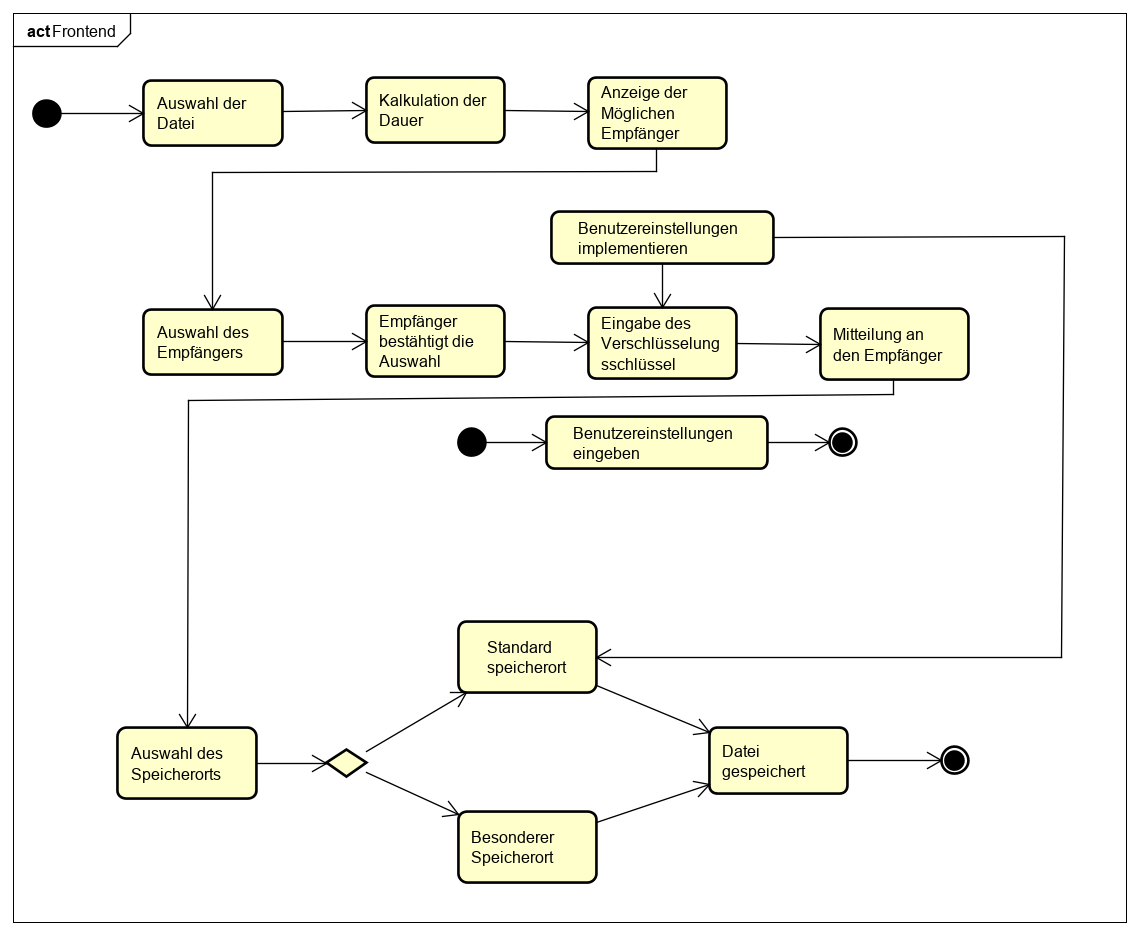
\includegraphics[width= 0.9\linewidth]{diagramms/activity/Frontend.png}
	\caption{Aktivitätsdiagramm Frontend}
\end{figure}
\newpage
\begin{indentE}\mbox{}
	\paragraph{/LF2210/ Datei auswählen}\mbox{}\\
	Der Benutzer wählt eine Datei aus, welche er verschicken möchte. Hierbei soll eine voreilige Kalkulation durchgeführt werden, welche die Dauer der Übertragung schätzt.
	\UseCase{
		{App Frontend}
		{/LF2210/ Datei auswählen}
		{Frontend}
		{Ein wird die zu versendende Datei ausgewählt.}
		{Es muss die Datei, welche versendet werden soll, ausgewählt werden}
		{Es kann die Datei gesendet werden}
		{Sender}
		{Datei(Name, Größe, Inhalt)}
		{Es kann keine Datei ausgewählt werden}
		{Es kann eine zu versendende Datei ausgewählt werden}
		{hoch}
		{mittel}
		{Should Have}
	}
	\paragraph{/LF2220/ Empfänger auswählen}\mbox{}\\
	Es werden dem Benutzer die möglichen Empfänger angezeigt und ausgwählt oder er kann den Namen des Empfängers eingeben, um den Empfänger zu bestimmen. Dieser muss die Verbindung bestätigen.
	\UseCase{
		{App Frontend}
		{/LF2220/ Empfänger auswählen}
		{Frontend}
		{Der Sender wählt anhand des Namens den Empfänger aus, mit dem der Datentransfer stattfinden soll.}
		{Es muss der Empfänger ausgewählt werden.}
		{Die Verbindung kann aufgebaut werden}
		{Sender, Empfänger}
		{Sendername, Empfängername}
		{Es kann kein Empfänger ausgewählt werden.}
		{Es kann anhand des Namens der Empfänger der Datei ausgewählt werden.}
		{hoch}
		{mittel}
		{Should Have}
	}
	\paragraph{/LF2230/ Verschlüsselungsschlüssel eingeben}\mbox{}\\
	Wenn kein Standard-Schlüssel ausgewählt ist, muss der Sender diesen bevor dem Verbindungsaufbau eingeben. Dieser muss dann dem Empfänger mitgeteilt werden und dieser muss den selben auch eingeben, um den Datentransfer zu ermöglichen.
	\UseCase{
		{App Frontend}
		{/LF2230/ Verschlüsselungsschlüssel eingeben}
		{Frontend}
		{Es müssen Empfänger und Sender einen Schlüssel eingeben, die übereinstimmen, um den Datentransfer zu beginnen.}
		{Der Datentransfer muss mit einem Schlüssel verschlüsselt werden.}
		{Der Datentransfer kann verschlüsselt werden}
		{Sender, Empfänger}
		{Schlüssel}
		{Die Daten können nicht mit einem Schlüssel verschlüsselt werden}
		{Die Daten können mit einem frei wählbaren Schlüssel verschlüsselt werden}
		{hoch}
		{mittel}
		{Should Have}
	}
	\paragraph{/LF2240/ Datei speichern}\mbox{}\\
	Der Empfänger soll nach dem empfangen der Datei auswählen können, ob diese im Standard-Speicherort gespeichert wird, oder in einem besonderen. Wenn der Besondere ausgewählt worden ist, soll ihm ein Benutzerinterface gezeigt werden, indem er den Speicherort auswählen.
	\UseCase{
		{App Frontend}
		{/LF2240/ Datei speichern}
		{Frontend}
		{Der Empfänger soll den Speicherort des bekommenen Datei auswählen können.}
		{Die Datei muss irgendwo gespeichert werden}
		{Der Speicherort der Datei kann ausgewählt werden}
		{Empfänger}
		{Datei(Name, Größe, Inhalt), Speicherort}
		{Die Datei wird entweder immer am selben Ort, oder nicht gespeichert}
		{Der Speicherort kann frei gewählt werden}
		{mittel}
		{gering}
		{Should Have}
	}
	\paragraph{/LF2250/ Benutzereinstellungen hinzufügen}\mbox{}\\
	Der Benutzer kann einige Fix-Einstellungen auf seinem Produkt tätigen. Darunter zählt die Möglichkeit, den Namen zu ändern, welcher den restlichen Nutzern angezeigt wird, die Verschlüsselung zu aktivieren oder deaktivieren, einen Standardschlüssel auszuwählen und einen Standard-Speicherort auszuwählen. Dabei sollen die eingegebenen Daten auf ihre Korrektheit überprüft werden.
	\UseCase{
		{App Frontend}
		{/LF2250/ Benutzereinstellungen hinzufügen}
		{Frontend}
		{Der Benutzer kann verschiedenen Einstellungen tätigen, mit welche er die Datenübertragung beeinflussen kann.}
		{Die Einstellungen müssen auf einem Interface getätigt werden}
		{Die Einstellungen können getätigt werden}
		{Empfänger, Sender}
		{gewünschter Systemname, Verschlüsselung(Ja/Nein), Standardschlüssel, Standard-Speicherort}
		{Das Produkt kann nicht angepasst werden.}
		{Es können Einstellungen getroffen werden, welche das Produkt beeinflussen.}
		{mittel}
		{mittel}
		{Nice to Have}
	}
	\paragraph{/LF2260/ Appinterface designen}\mbox{}\\
	Es muss ein Interface für das Smartphone entworfen werden. Dazu gehören Mockups und Prototypen. Diese müssen vor deren Implementierung vom Auftraggeber bestätigt werden.
	\UseCase{
		{App Frontend}
		{/LF2260/ Appinterface designen}
		{Frontend}
		{Es müssen Mockups für die Appinterfaces erstellt werden. Diese diene als Vorlage für die Interfaces.}
		{Für einen schnellere und besser Implementierung sollen Mockups als Vorlage dienen.}
		{Die Implementierung ist einfacher, schneller und besser.}
		{Auftraggeber, Auftragnehmer}
		{}
		{Das Interface wird ohne Vorlage erstellt.}
		{Das Interface kann nach einer vom Auftraggeber bestätigten Vorlage erstellt werden.}
		{mittel}
		{gering}
		{Nice to Have}
	}
	\paragraph{/LF2270/ Appinterface implementieren}\mbox{}\\
	Das Appinterface muss nach der Bestätigung des Auftraggeber implementiert werden. 
	\UseCase{
		{App Frontend}
		{/LF2270/ Appinterface implementieren}
		{Frontend}
		{Das Appinterface muss durch die Mockups realisiert werden.}
		{Der Benutzer hat keine Möglichkeit mit dem System zu integrieren}
		{Der Benutzer kann mit dem System interagieren und dadurch dessen Funktionen benutzen.}
		{Benutzer}
		{sämtliche Nutzereingaben}
		{Der Benutzer kann mit dem System nicht interagieren}
		{Der Benutzer ist in der Lage mit dem System zu interagieren}
		{hoch}
		{hoch}
		{Should Have}
	}
	\paragraph{/LF2280/ Frontend und Backend verbinden}\mbox{}\\
	Es muss eine Verbindung zwischen dem Frontend und Backend erstellt werden, welche die Aufforderungen verarbeitet und zum Backend weiterleitet. Diese Verbindung, soll dem Benutzer entweder mitteilen, wie lange die Verarbeitung noch dauert oder bei kürzeren das wiederholte Aufrufen von Aufforderungen verhindern.
	\UseCase{
		{App Frontend}
		{/LF2280/ Frontend und Backend verbinden}
		{Frontend}
		{Das Frontend muss mit dem Backend verbunden werden, um die Nutzereingaben an das Backend weiterzuleiten. Außerdem soll es Daten ans Frontend schicken, welche über momentane Prozess aufklärt.}
		{Die Daten müssen vom Frontend ans Backend und umgekehrt geschickt werden}
		{Das Frontend kann mit dem Backend und umgekehrt kommunizieren.}
		{Benutzer}
		{sämtliche Nutzereingaben und verwertete Daten}
		{Die Nutzerdaten können nicht an das Backend und die verwerteten Daten nicht ans Frontend geschickt werden.}
		{Daten können zwischen Frontend und Backend ausgetauscht werden.}
		{hoch}
		{mittel}
		{Should Have}
	}
\end{indentE}
\subsection{Publizierung}
Um mit dem Produkt etwas zu erwirtschaften, muss dieses der Zielgruppe anschaulich gemacht werden. Dabei ist die größe der Plattformen und die Anzahl der Plattformen, welche dies machen, für ein erfolgreiches Produkt besonders wichtig.
\paragraph{Aktivitätsdiagramm Publizierung}\mbox{}\\
\begin{figure}[H]
	\centering
	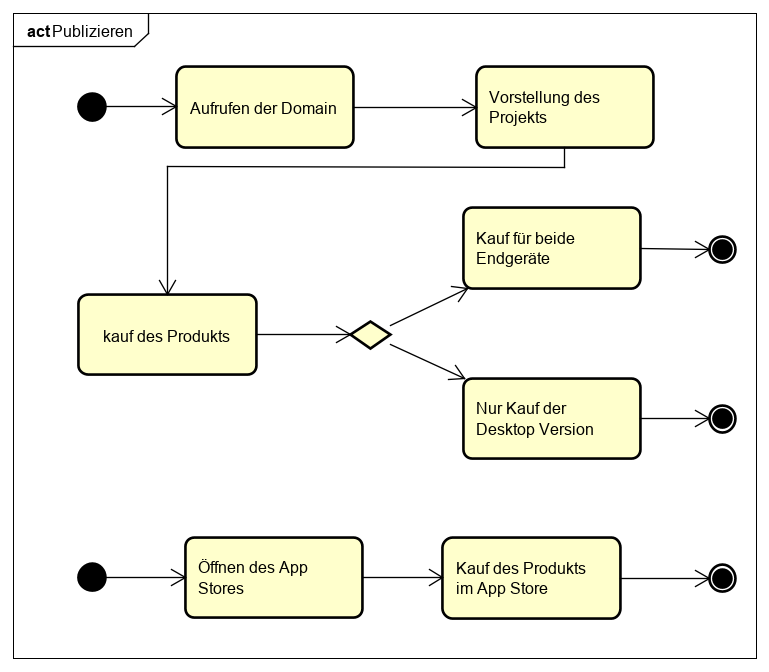
\includegraphics[width= 0.9\linewidth]{diagramms/activity/Publizieren.png}
	\caption{Aktivitätsdiagramm Publizierung}
\end{figure}
\newpage
\begin{indentE}\mbox{}
	\paragraph{/LF3110/ Website erstellen}\mbox{}\\
	Es wird eine Webseite erstellt, auf welche das Produkt vorgestellt wird. Außerdem soll diese dem Besucher das Projektteam und den Auftraggeber näher bringen, auf einer eigenen About-Seite. Diese Webseite wird dann auf einen Hosting-Provider hochgeladen, von wo sie mit einer Domain aufgerufen werden kann.
	\UseCase{
		{Publizierung}
		{/LF3110/ Website erstellen}
		{Publizierung}
		{Es wird eine Webseite erstellt, auf welche das Produkt publiziert werden soll. Diese soll außerdem auf das Projektteam aufmerksam machen und über das Internet mit einer Domain erreichbar sein.}
		{Das Produkt soll auf einer Webseite publiziert werden, und den potenziellen Kunden das Projektteam näher gebracht werden.}
		{Das Produkt ist im Internet auffindbar}
		{Benutzer, Projektteam (Auftraggeber + Auftragnehmer)}
		{Produktinformationen, Projektteam}
		{Das Produkt kann nicht über eine Webseite aufgefunden werden.}
		{Das Produkt ist über ein Webseite auffindbar}
		{hoch}
		{gering}
		{Must Have}
	}
	\paragraph{/LF3120/ Produkt auf Webseite veröffentlichen}\mbox{}\\
	Das Produkt muss auf ihrer eigenen Webseite /LF2060/ publiziert werden. Diese besitzt eine eigne Seite für den Download der Software. Dort kann man die App und Desktop Version für 5€ kaufen und die Desktop Version einzeln für 3€.
	\UseCase{
		{Publizierung}
		{LF3120/ Produkt auf Webseite veröffentlichen}
		{Publizierung}
		{Das Produkt soll von der Webseite gedownloadet werden können. Dabei soll die App und Desktop Version für 5 € gemeinsame und die Desktop Version einzeln für 3€ angeboten werden.}
		{Das Produkt muss für den potenziellen Kunden erwerbbar sein}
		{Das Produkt kann auf der Webseite automatisiert verkauft werden}
		{potenzieller Kunde}
		{Zahlungsinformationen, Produkt (als Download)}
		{Das Produkt ist für den potenziellen Kunden nicht erwerbbar}
		{Das Produkt kann auf der Webseite verwirtschaftet werden}
		{hoch}
		{mittel}
		{Must Have}
	}
	\paragraph{/LF3210/ Produkt auf Play Store veröffentlichen}\mbox{}\\
	Die Android App soll auf dem Google Play Store hochgeladen werden und dort für eine Preis von 3€ verkauft werden. Dafür muss ein Google Developer Account erstellt werden, um diese hochzuladen.
	\UseCase{
		{Publizierung}
		{/LF3210/ Produkt auf Play Store veröffentlichen}
		{Publizierung}
		{Die App-Version wird auf dem Play Store veröffentlicht, wo sie für 3€ erwerbt werden kann.}
		{Es soll die potenzielle Kundschaft erhöht werden, indem ie App-Version auch auf dem Play-Store verfügbar ist.}
		{Es wird eine größter Kundschaft(Android) angesprochen}
		{potenzielle Kunden}
		{App-Version(als Download)}
		{Der Erwerb wird nicht auf dem Play Store angeboten.}
		{Der Erwerb ist über den Play Store möglich}
		{mittel}
		{gering}
		{Should Have}
	}
	\paragraph{/LF3220/ Produkt auf App Store veröffentlichen}\mbox{}\\
	Die iOS App kann auf dem Apple App Store hochgeladen werden und dort für 3€ verkauft werden.
	\UseCase{
		{Publizierung}
		{/LF3220/ Produkt auf App Store veröffentlichen}
		{Publizierung}
		{Die App-Version wird auf dem App Store veröffentlicht, wo sie für 3€ erwerbt werden kann.}
		{Es soll die potenzielle Kundschaft erhöht werden, indem ie App-Version auch auf dem App Store verfügbar ist.}
		{Es wird eine größter Kundschaft(iOS) angesprochen}
		{potenzielle Kunden}
		{App-Version(als Download)}
		{Der Erwerb wird nicht auf dem App Store angeboten.}
		{Der Erwerb ist über den App Store möglich}
		{mittel}
		{mittel}
		{Nice to Have}
	}
\end{indentE} %Georg & Luca
	\newpage
	\section{Produktdaten}
Das Endprodukt muss für die erfolgreiche Verwendung auf einige Benutzerdaten zugreifen können und diese in manchen Fällen sogar verändern. Außerdem müssen Daten für den Transfer kurzzeitig gespeichert und mit dem Empfänger mit jedem Paket ausgetauscht werden.
\\
%\begin{comment}
\begin{figure}[H]
	\centering
	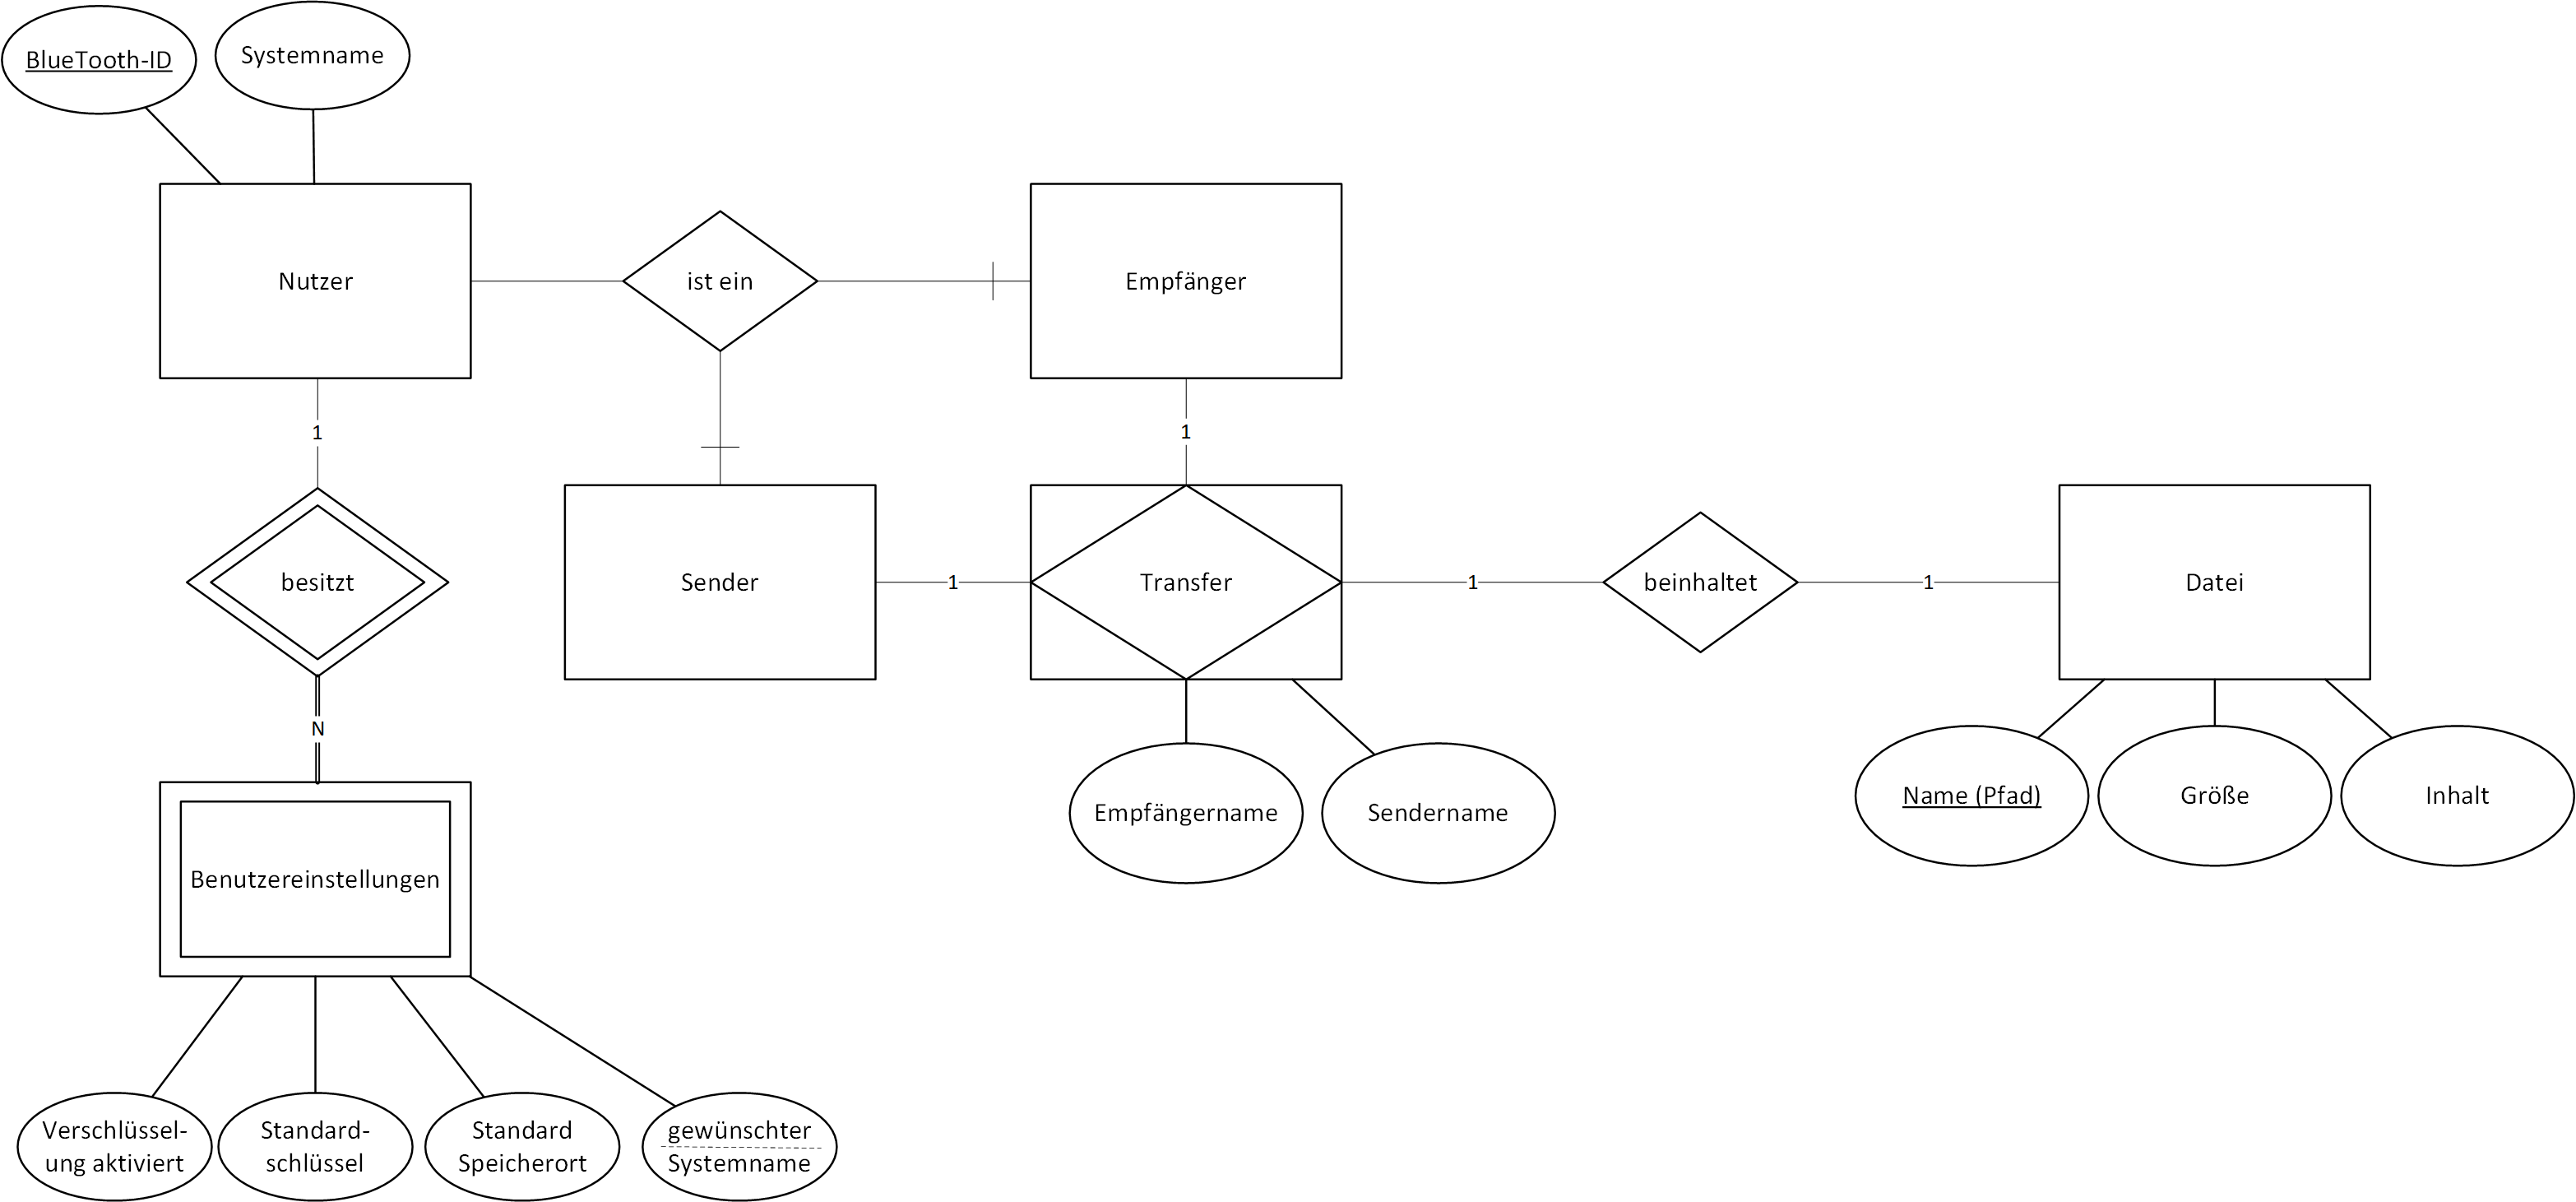
\includegraphics[width=\linewidth]{diagramms/erd/erd.png}\
	\caption{ERD}
\end{figure}
\newpage
%\end{comment}
\subsection{/LD1000/ Systemdaten}
\begin{itemize}
	\item momentaner-Systemname
	\item BlueTooth-Version
\end{itemize}
\subsection{/LD2000/ Datei}
\begin{itemize}
	\item Dateiname
	\item Dateigröße
	\item Dateiinhalt
\end{itemize}
\subsection{/LD3000/ Transferdaten}
\begin{itemize}
	\item Sendername
	\item Empfängername
	\item Datei
	\item Index Paket
	\item Anzahl Pakete
\end{itemize}
\subsection{/LD4000/ Benutzereinstellungen}
\begin{itemize}
	\item gewünschter Systemname
	\item Verschlüsselung (de- oder aktiviert)
	\item Standardschlüssel
	\item Standard-Speicherort
\end{itemize} %Florian	
	\newpage
	\section{Produktleistungen}
Diese Leistungen, müssen vom Produkt erfüllt werden, damit diesen vom Auftraggeber angenommen wird. Sind diese nicht erfüllt, darf der Auftraggeber den Abschluss des Projektes als verhindern.
\begin{indentE}\mbox{}
	\paragraph{/L1010/ Produktgröße}\mbox{}\\
	Die Gesamtgröße des Endprodukt soll für ein System nicht größer sein als 500MB. Das heißt, das weder die App noch Desktopversion eine Größe von 500MB überschreiten darf. Der Grund dafür ist, das eine Anwendung über dieser Größe potenzielle Nutzer abschrecken könnte, da diese nicht mehr als 500MB an speicher freimachen wollen.
	\paragraph{/L1020/ Empfänger anzeigen}\mbox{}\\
	Das anzeigen aller Empfänger in einem Radius von 5m (ohne Hindernisse) soll einer Dauer von 10 Sekunden nicht überschreiten.
	\paragraph{/L1030/ Verbindungsaufbauzeit}\mbox{}\\
	Der Verbindungsaufbau zwischen dem Sender und Empfänger soll mit Android 8 oder mit einem Intel 7th Gen CPU ausgerüsteten Geräten eine Dauer von 30 Sekunden (exklusive Benutzereingaben) dauern
	\paragraph{/L1040/ Datenübertragungsrate}\mbox{}\\
	Es soll mit dem Produkt möglich sein mit einer Datentransferrate von bis zu 25 Mbit/s mit Bluetooth Version 5.0 Daten zu übertragen, diese kann bei jüngeren Bluetooth Versionen geringer sein.
	\paragraph{/L1050/ Dateigröße}\mbox{}\\
	Das Produkt sollen Daten bis zu einer Größen von 1GB problemlos übertragen werden können.
	\paragraph{/L2110/ Windows kompatibel}\mbox{}\\
	Das System muss für Windows 10 kompatibel sein, und auf diesen Betriebssystem mit all seinen Funktionen funktionieren.
	\paragraph{/L2120/ Debian kompatibel}\mbox{}\\
	Das System sollte für Debian 9 kompatibel sein, und auf diesen Betriebssystem mit all seinen Funktionen funktionieren.
\end{indentE} %Georg 
	\newpage
	\section{Benutzungsschnittstellen}
Es werden Visuelle Darstellungen der Benutzerschnittstellen von der Desktop-Applikation als auch Smartphone-Version gezeigt.
\subsection{Desktop}
Es folgen die Mockups zu der Desktop-Applikationen. Diese dienen als Vorlage für die tatsächliche Realisierung für das Produkt.
\subsubsection{Home Screen}
\begin{figure}[H]
	\centering
	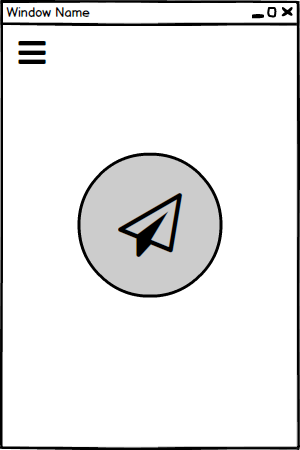
\includegraphics[width=.7\linewidth]{pictures/Desktop/Home.png}\
	\caption{Home Screen der Desktop-Applikation}
\end{figure}
Die Desktop-Applikation soll nicht all zu viel Platz einnehmen weswegen die Größe auf 300 Pixel x 450 Pixel beschränkt wurde. Wie bereits erwähnt gibt es ein simples GUI mit dem man mit nur einem Knopfdruck eine Datei auswählen kann. Ebenfalls hat der Benutzer jederzeit zugriff auf die Optionen welche Links oben mit einem Burger-Menü angezeigt werden.
\subsubsection{Verschlüsselungskey eingeben}
\begin{figure}[H]
	\centering
	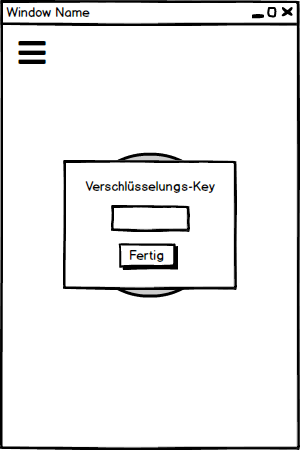
\includegraphics[width=.7\linewidth]{pictures/Desktop/Verschluesselungskey.png}\
	\caption{Eingabefeld des Verschlüsselungskey}
\end{figure}
Bevor dieser Schritt ausgeführt werden kann und der Benutzer zu dieser Schnittstelle kommt muss er, in dem vom Betriebssystem geöffneten File Explorer, die zu versendende Datei auswählen. Wenn dies erfüllt ist kann man einen individuellen Verschlüsselungskey eingegeben werden, welcher dann bei dem Empfänger zur Entschlüsselung der Daten gebraucht wird. Falls sich der Benutzer dazu entscheidet keinen eigenen Schlüssel einzugeben wird der Standardschlüssel, welcher in den Einstellungen zu finden ist, verwendet. In beiden Fällen muss der Benutzer mit einem Knopfdruck auf den "Fertig"-Knopf die Eingabe bestätigen.
\subsubsection{Empfänger auswählen}
\begin{figure}[H]
	\centering
	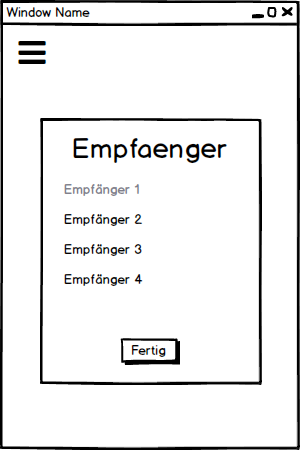
\includegraphics[width=.7\linewidth]{pictures/Desktop/Empfaenger.png}\
	\caption{Empfänger auswählen}
\end{figure}
Nachdem der Schlüssel erfolgreich eingegeben wurde kann der Benutzer nun einen Empfänger auswählen. Hierbei werden ihm alle möglichen Geräte, welche in der Empfangsreichweite sind, angezeigt. Mit einem Knopfdruck auf den Empfängernamen wird er ausgewählt. Dies ist an der Änderung der Farbe erkennbar welche von Schwarz zu Grau wird. Auch hier muss die Auswahl bestätigt werden was mit einem Klick auf den "Fertig"-Knopf getan wird.
\subsubsection{Fortschrittsbalken anzeigen}
\begin{figure}[H]
	\centering
	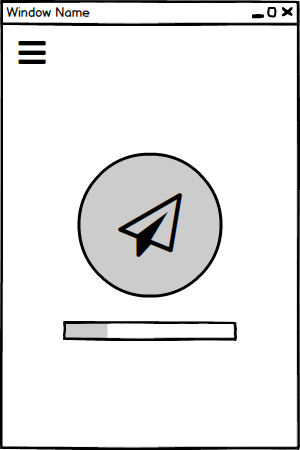
\includegraphics[width=.7\linewidth]{pictures/Desktop/Progress.png}\
	\caption{Fortschrittsbalken anzeigen}
\end{figure}
Wenn nun alle Kriterien für eine erfolgreiche Datenübertragung getroffen wurden, wird die Datei an den zuvor ausgewählten Empfänger gesendet. Dieser Schritt wird auch mit einem Fortschrittsbalken dargestellt.
\subsubsection{Optionen anzeigen}
\begin{figure}[H]
	\centering
	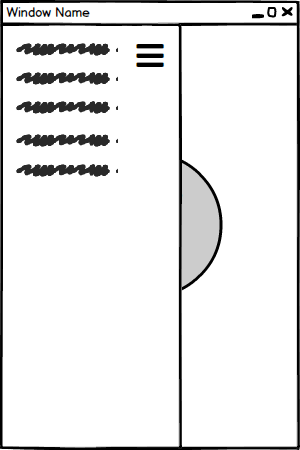
\includegraphics[width=.7\linewidth]{pictures/Desktop/Options.png}\
	\caption{Optionen anzeigen}
\end{figure}
Falls der Benutzer etwas an den Einstellungen ändern möchte, kann dieser zu jedem Zeitpunkt Links oben in der Applikation auf das Burger-Menü klicken was zu einem anzeigen der Optionen führt. Auf der Linken Seite werden dann mehrere Auswahlmöglichkeiten angezeigt. Mit einem Klick auf eine der Optionen komm der Benutzer auf eine neue Seite, wo dann die, zur Einstellung passenden, Informationen angezeigt werden. Um das Menü wieder verschwinden zu lassen kann der Benutzer entweder außerhalb des Optionen Feld klicken oder erneut auf das Burger-Menü drücken. 
\subsubsection{Einstellungen anzeigen}
\begin{figure}[H]
	\centering
	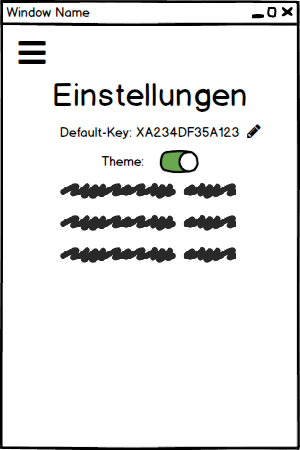
\includegraphics[width=.7\linewidth]{pictures/Desktop/Einstellungen.png}\
	\caption{Einstellungen anzeigen}
\end{figure}
Ein wichtiger Unterpunkt welcher in den Optionen zu sehen ist, sind die Einstellungen. In diesen kann man zum Beispiel den Default-Key sehen oder bei bedarf sogar verändern. Ebenfalls gibt es noch andere Einstellungen welche derzeit mit einem Placeholder belegt sind. Um aus den Einstellungen wieder zum Home Screen zu kommen muss der Benutzer das Burger Menü öffnen auf den Unterpunkt "Home" klicken.
\subsubsection{Nachrichten}
\begin{figure}[H]
	\centering
	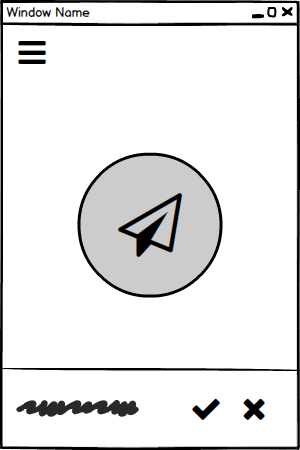
\includegraphics[width=.7\linewidth]{pictures/Desktop/Nachricht.png}\
	\caption{Nachrichten}
\end{figure}
Wenn der Sender nun einen Empfänger ausgewählt hat, erhält dieser eine Nachricht. Diese wird am unteren Rand der Applikation angezeigt und beinhaltet Informationen zum Dateinamen. Neben den Informationen hat der Benutzer 2 Optionen. Das Check Symbol signalisiert das Annehmen der Datei, das Kreuz das Ablehnen. Wenn sich der Benutzer entschieden hat ob er die Datei annehmen oder ablehnen möchte, klickt er einfach auf eines der Symbole. Bei klicken des Kreuzes verschwindet die Nachricht und die Datei kann nicht mehr heruntergeladen werden. Bei anklicken des Check Symbols kommt es zu der nächsten Schnittstelle.
\subsubsection{Nachricht akzeptieren}
\begin{figure}[H]
	\centering
	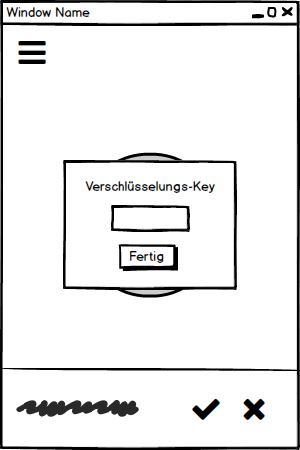
\includegraphics[width=.7\linewidth]{pictures/Desktop/Nachrichtaccept.png}\
	\caption{Nachricht akzeptieren}
\end{figure}
Hat der Empfänger sich dazu entschieden die Datei anzunehmen, kommt wie zuvor schon erwähnt ein Eingabefeld in welchem der gewählte Verschlüsselungskey einzugeben ist. Wenn dieser erfolgreich eingegeben wird und mit einem Klick auf den "Fertig"-Knopf bestätigt wird, wird die übertragene Datei heruntergeladen und kann nun auf dem Gerät des Empfängers geöffnet werden. Gibt es einen Fehler bei der Eingabe des Verschlüsselungskey hat der Benutzer erneut die Chance diesen einzugeben.

\subsection{Smartphone}
Es folgen die Mockups zu der Smartphone-Version der Applikation. Diese dienen als Vorlage für die tatsächliche Realisierung für das Produkt.
\subsubsection{Home Screen}
\begin{figure}[H]
	\centering
	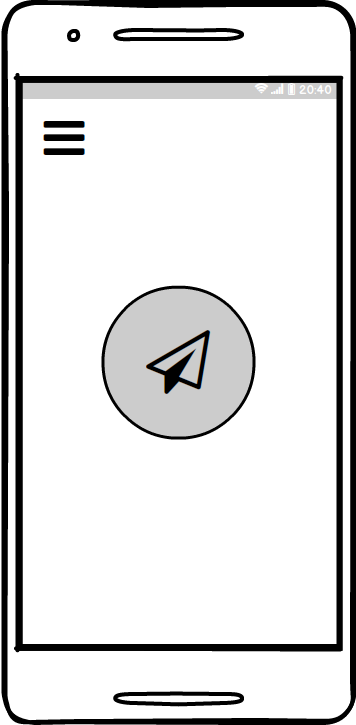
\includegraphics[width=.5\linewidth]{pictures/Mobile/Home.png}\
	\caption{Home Screen der Desktop-Applikation}
\end{figure}
Die Desktop-Applikation soll nicht all zu viel Platz einnehmen weswegen die Größe auf 300 Pixel x 450 Pixel beschränkt wurde. Wie bereits erwähnt gibt es ein simples GUI mit dem man mit nur einem Knopfdruck eine Datei auswählen kann. Ebenfalls hat der Benutzer jederzeit zugriff auf die Optionen welche Links oben mit einem Burger-Menü angezeigt werden.
\subsubsection{Verschlüsselungskey eingeben}
\begin{figure}[H]
	\centering
	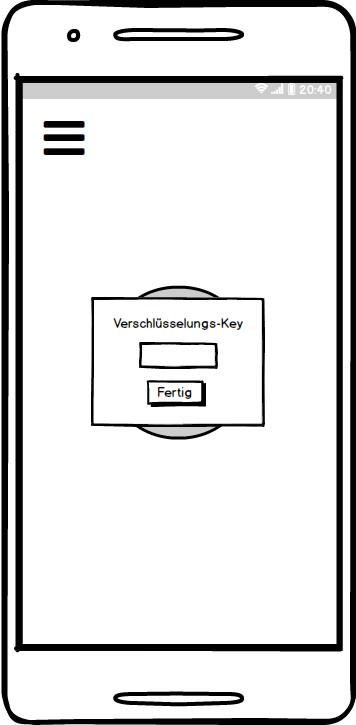
\includegraphics[width=.5\linewidth]{pictures/Mobile/Verschluesselungskey.png}\
	\caption{Eingabefeld des Verschlüsselungskey}
\end{figure}
Bevor dieser Schritt ausgeführt werden kann und der Benutzer zu dieser Schnittstelle kommt muss er, in dem vom Betriebssystem geöffneten File Explorer, die zu versendende Datei auswählen. Wenn dies erfüllt ist kann man einen individuellen Verschlüsselungskey eingegeben werden, welcher dann bei dem Empfänger zur Entschlüsselung der Daten gebraucht wird. Falls sich der Benutzer dazu entscheidet keinen eigenen Schlüssel einzugeben wird der Standardschlüssel, welcher in den Einstellungen zu finden ist, verwendet. In beiden Fällen muss der Benutzer mit einem Knopfdruck auf den "Fertig"-Knopf die Eingabe bestätigen.
\subsubsection{Empfänger auswählen}
\begin{figure}[H]
	\centering
	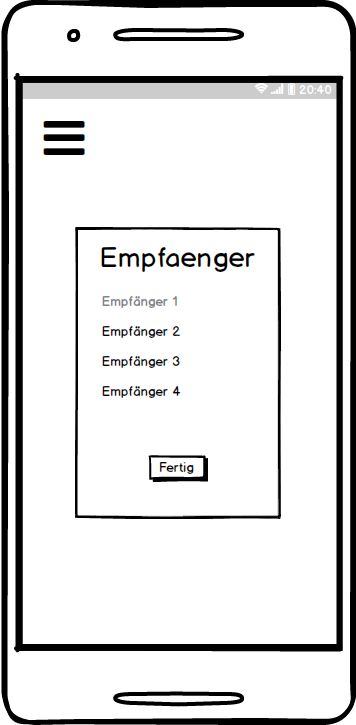
\includegraphics[width=.5\linewidth]{pictures/Mobile/Empfaenger.png}\
	\caption{Empfänger auswählen}
\end{figure}
Nachdem der Schlüssel erfolgreich eingegeben wurde kann der Benutzer nun einen Empfänger auswählen. Hierbei werden ihm alle möglichen Geräte, welche in der Empfangsreichweite sind, angezeigt. Mit einem Knopfdruck auf den Empfängernamen wird er ausgewählt. Dies ist an der Änderung der Farbe erkennbar welche von Schwarz zu Grau wird. Auch hier muss die Auswahl bestätigt werden was mit einem Klick auf den "Fertig"-Knopf getan wird.
\subsubsection{Fortschrittsbalken anzeigen}
\begin{figure}[H]
	\centering
	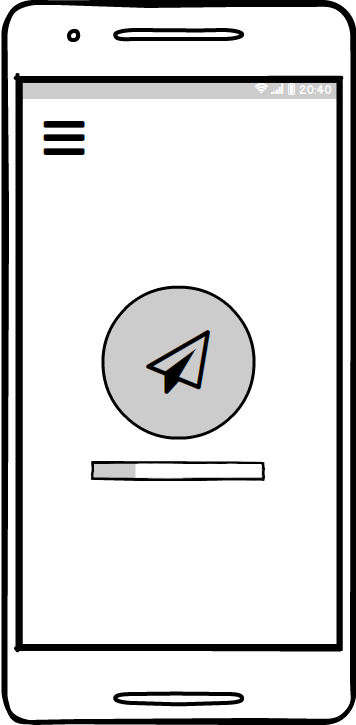
\includegraphics[width=.5\linewidth]{pictures/Mobile/Progress.png}\
	\caption{Fortschrittsbalken anzeigen}
\end{figure}
Wenn nun alle Kriterien für eine erfolgreiche Datenübertragung getroffen wurden, wird die Datei an den zuvor ausgewählten Empfänger gesendet. Dieser Schritt wird auch mit einem Fortschrittsbalken dargestellt.
\subsubsection{Optionen anzeigen}
\begin{figure}[H]
	\centering
	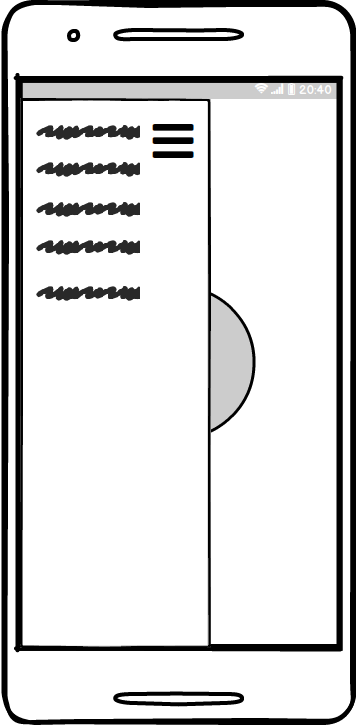
\includegraphics[width=.5\linewidth]{pictures/Mobile/Options.png}\
	\caption{Optionen anzeigen}
\end{figure}
Falls der Benutzer etwas an den Einstellungen ändern möchte, kann dieser zu jedem Zeitpunkt Links oben in der Applikation auf das Burger-Menü klicken was zu einem anzeigen der Optionen führt. Auf der Linken Seite werden dann mehrere Auswahlmöglichkeiten angezeigt. Mit einem Klick auf eine der Optionen komm der Benutzer auf eine neue Seite, wo dann die, zur Einstellung passenden, Informationen angezeigt werden. Um das Menü wieder verschwinden zu lassen kann der Benutzer entweder außerhalb des Optionen Feld klicken oder erneut auf das Burger-Menü drücken. 
\subsubsection{Einstellungen anzeigen}
\begin{figure}[H]
	\centering
	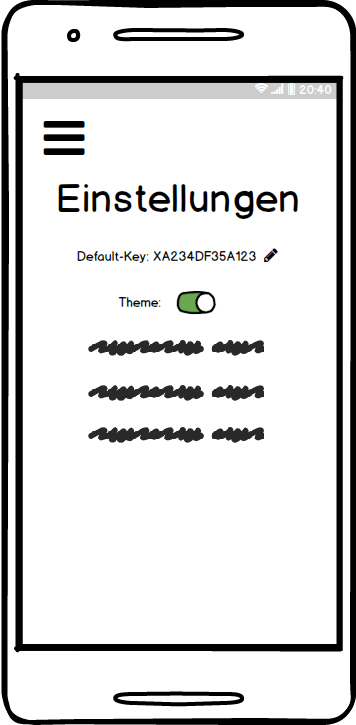
\includegraphics[width=.5\linewidth]{pictures/Mobile/Einstellungen.png}\
	\caption{Einstellungen anzeigen}
\end{figure}
Ein wichtiger Unterpunkt welcher in den Optionen zu sehen ist, sind die Einstellungen. In diesen kann man zum Beispiel den Default-Key sehen oder bei bedarf sogar verändern. Ebenfalls gibt es noch andere Einstellungen welche derzeit mit einem Placeholder belegt sind. Um aus den Einstellungen wieder zum Home Screen zu kommen muss der Benutzer das Burger Menü öffnen auf den Unterpunkt "Home" klicken.
\subsubsection{Nachrichten}
\begin{figure}[H]
	\centering
	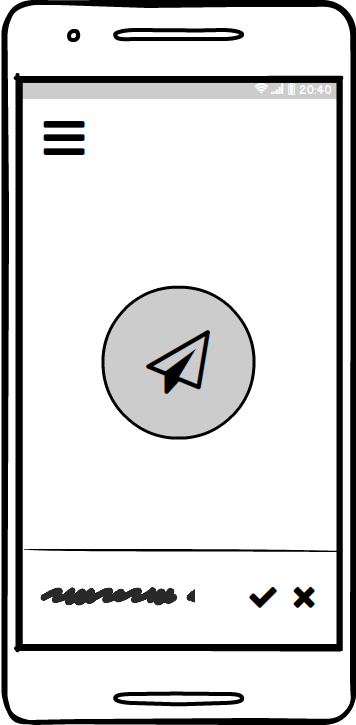
\includegraphics[width=.5\linewidth]{pictures/Mobile/Nachricht.png}\
	\caption{Nachrichten}
\end{figure}
Wenn der Sender nun einen Empfänger ausgewählt hat, erhält dieser eine Nachricht. Diese wird am unteren Rand der Applikation angezeigt und beinhaltet Informationen zum Dateinamen. Neben den Informationen hat der Benutzer 2 Optionen. Das Check Symbol signalisiert das Annehmen der Datei, das Kreuz das Ablehnen. Wenn sich der Benutzer entschieden hat ob er die Datei annehmen oder ablehnen möchte, klickt er einfach auf eines der Symbole. Bei klicken des Kreuzes verschwindet die Nachricht und die Datei kann nicht mehr heruntergeladen werden. Bei anklicken des Check Symbols kommt es zu der nächsten Schnittstelle.
\subsubsection{Nachricht akzeptieren}
\begin{figure}[H]
	\centering
	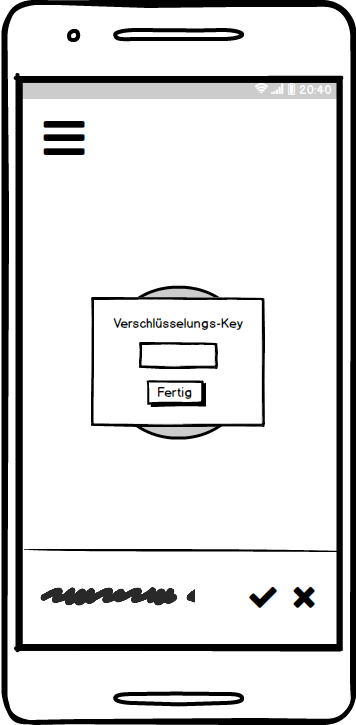
\includegraphics[width=.5\linewidth]{pictures/Mobile/Nachrichtaccept.png}\
	\caption{Nachricht akzeptieren}
\end{figure}
Hat der Empfänger sich dazu entschieden die Datei anzunehmen, kommt wie zuvor schon erwähnt ein Eingabefeld in welchem der gewählte Verschlüsselungskey einzugeben ist. Wenn dieser erfolgreich eingegeben wird und mit einem Klick auf den "Fertig"-Knopf bestätigt wird, wird die übertragene Datei heruntergeladen und kann nun auf dem Gerät des Empfängers geöffnet werden. Gibt es einen Fehler bei der Eingabe des Verschlüsselungskey hat der Benutzer erneut die Chance diesen einzugeben. %Markus
	\newpage
	\section{Qualitätsbestimmung}
Es wird das Produkt anhand der zu erbringenden Qualitäten beschrieben. Diese Qualitäten werden anhand dessen Auswirkung auf das Projekt einzeln beschreibend

\begin{table}[H]
	\begin{center}
		\begin{tabularx}{\linewidth}{|X|c|c|c|c|}
			\hline
			\textbf{Produktqualität}&Sehr gut&Gut&Normal&Nicht relevant\\
			\hline
			Funktionalität&X&&&\\
			\hline
			Angemessenheit&&&X&\\
			\hline
			Richtigkeit&X&&&\\
			\hline
			Interoperabilität&X&&&\\
			\hline
			Ordnungsmäßigkeit&X&&&\\
			\hline
			Sicherheit&&X&&\\
			\hline
			Zuverlässigkeit&&X&&\\
			\hline
			Reife&&&&X\\
			\hline
			Fehlertoleranz&&X&&\\
			\hline
			Wiederherstellbarkeit&&&X&\\
			\hline
			Benutzbarkeit&X&&&\\
			\hline
			Verständlichkeit&X&&&\\
			\hline
			Erlernbarkeit&&X&&\\
			\hline
			Bedienbarkeit&&X&&\\
			\hline
			Effizienz&&&X&\\
			\hline
			Zeitverhalten&&&X&\\
			\hline
			Verbrauchsverhalten&&&&X\\
			\hline
			Änderbarkeit&&X&&\\
			\hline
			Analysierbarkeit&&&&X\\
			\hline
			Modifizierbarkeit&&X&&\\
			\hline
			Stabilität&&&X&\\
			\hline
		\end{tabularx}
	\end{center}
\end{table}

\paragraph{Funktionalität}Es wird auf die Funktionen bezogenen und wie gut diese umgesetzt werden müssen
\paragraph{Angemessenheit}Es wird auf den Aufwand bezogenen und wie groß dieser sein soll zu Benutzung
\paragraph{Richtigkeit}Es wird auf die Richtigkeit(Komplettheit) der transferierten Daten bezogen
\paragraph{Interoperabilität}Es wird sich auf die Kompatibilität der Produktes mit verschiedenen Plattformen bezogen
\paragraph{Ordnungsgemäß}Es wird auf die Anzahl der Fehler bezogen, welche während der Sitzung aufkommen können
\paragraph{Sicherheit}Es wird sich auf die Sicherheit des Datentransfers bezogen
\paragraph{Zuverlässigkeit}Es wird sich auf die Zuverlässig Datenübertragung (keine Abbrüche) bezogen
\paragraph{Reife}Es wird sich auf die Qualität des Projektcodes bezogen
\paragraph{Fehlertoleranz}Es wird sich auf die Fähigkeit bezogen Fehler zu erkennen und richtig zu verwerten (kein Programmabsturz)
\paragraph{Wiederherstellbarkeit}Es wird sich auf die Wiederherstellbarkeit der Daten bei fehlerhaften Datentransfer bezogen
\paragraph{Benutzbarkeit}Es wird sich auf die Fähigkeit bezogen die Anwendung mit so wenigen Aktionen wie möglich zu bedienen
\paragraph{Verständlichkeit}Es werden sich auf Hilfsnachrichten bezogen, welche dem Benutzer bei der Verwendung helfen
\paragraph{Erlernbarkeit}Es wird sich auf die Möglichkeit bezogene das Programm ohne lesen der Hilfsnachrichten zu benutzen
\paragraph{Bedienbarkeit}Es wird sich auf die Bedienbarkeit aufgrund der benutzten Sprache im Programm bezogen
\paragraph{Effizienz}Es wird sich auf die Effizienz der vom Programm vollbrachten Funktionen bezogen anhand Ausführungszeit
\paragraph{Zeitverhalten}Es wird sich auf die Möglichkeit bezogen das Programm in naher Zukunft weiter zu benutzen
\paragraph{Verbrauchsverhalten}Es wird sich auf die vom Programm benötigten Ressourcen bezogen
\paragraph{Änderbarkeit}Es wird sich auf die Personalisierbarkeit des Programmes and den individuellen Benutzer bezogen
\paragraph{Stabilität}Es wird sich auf die Abstürze des Programms bezogen
 %Georg
	\newpage
	\section{Globale Testfälle}
Es werden die Fälle anhand von UseCase visualisiert, welche bei der Interaktion von Produkt externen Einflüssen passieren.
\\
\paragraph{Akteure}\mbox{}\\
\begin{figure}[H]
	\centering
	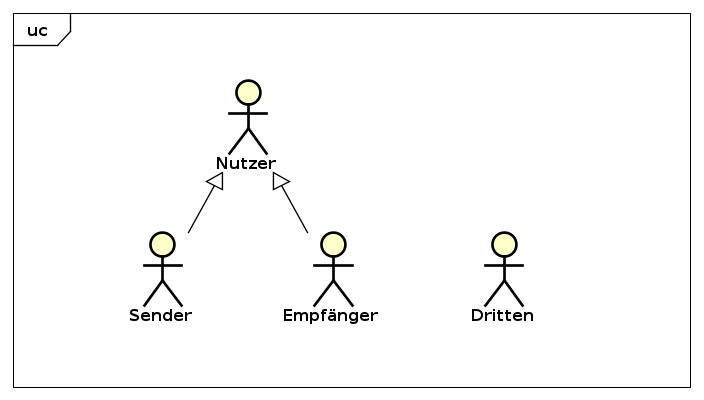
\includegraphics[width= 0.9\linewidth]{diagramms/useCase/akteure.png}
	\caption{Akteure}
\end{figure}
In der Abbildung 22, sind alle Akteure die in den folgenden Use-Case-Diagrammen vorkommen abgebildet. Hierbei gibt es einen Nutzer welcher sowohl ein Sender als auch ein Empfänger sein kann. Darüber hinaus gibt es Dritte welche in den Use-Cases mögliche Bedrohungen darstellt.
\newpage
\paragraph{Datentransfer}\mbox{}\\
\begin{figure}[H]
	\centering
	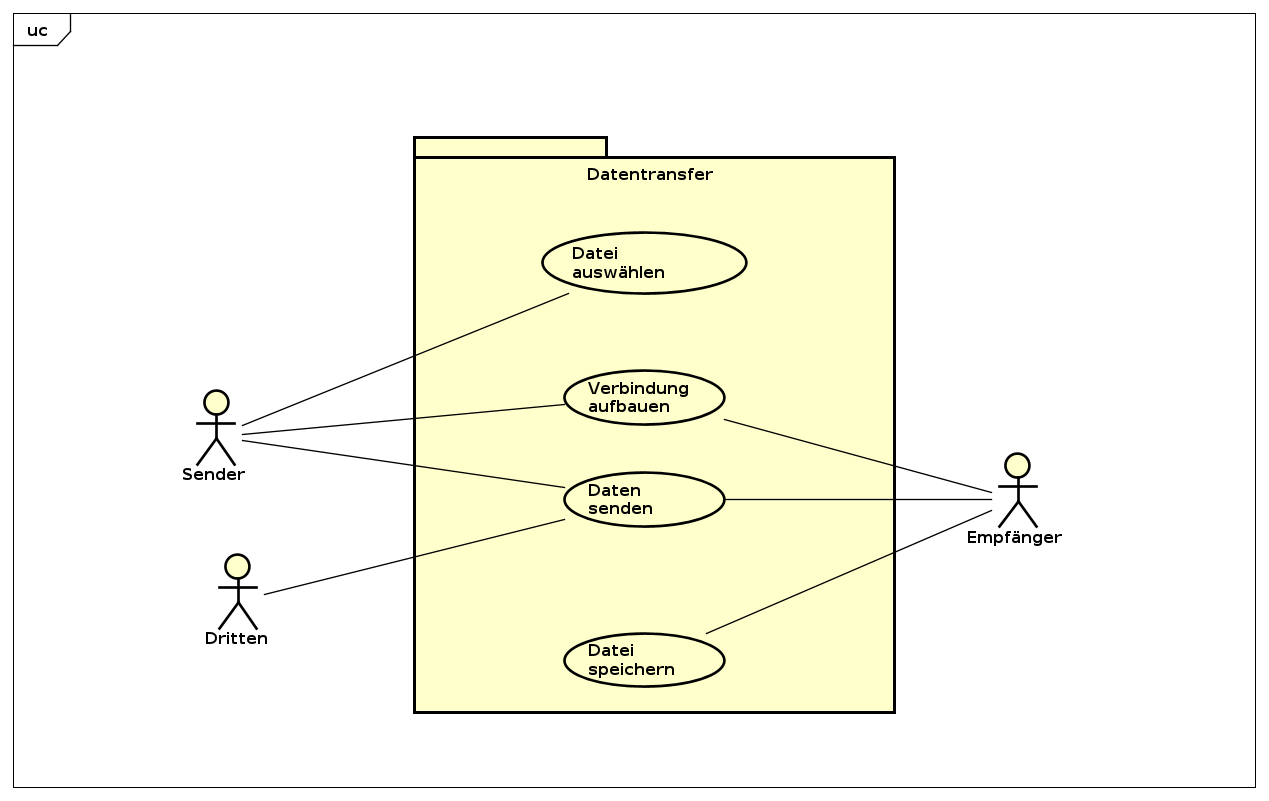
\includegraphics[width= 0.9\linewidth]{diagramms/useCase/datentransfer.png}
	\caption{Datentransfer}
\end{figure}
In der Abbildung wird der Grobe Datentransfer beschrieben. Hierbei ist jedes Use-Case auf den folgenden Seiten genauer vorgeführt und erklärt.
\newpage
\paragraph{Datei auswählen}\mbox{}\\
\begin{figure}[H]
	\centering
	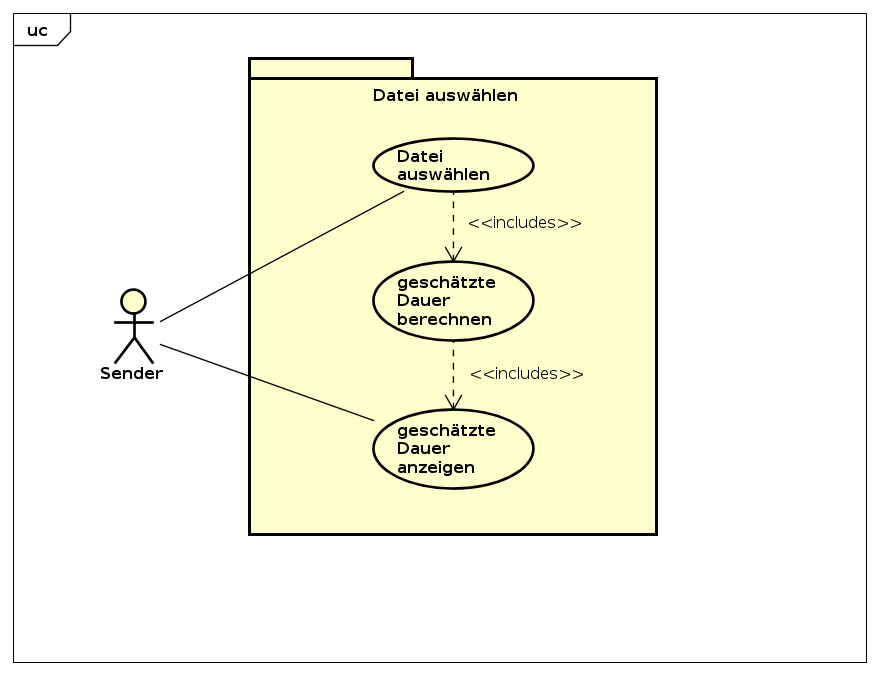
\includegraphics[width= 0.9\linewidth]{diagramms/useCase/datei_auswaehlen.png}
	\caption{Datei auswählen}
\end{figure}
Wenn der Sender auf den, im Mockup gezeigten, Knopf drückt öffnet sich der File Explorer wo man dann eine Datei auswählen kann. Nachdem die Datei ausgewählt wurde wird die geschätzte Dauer, welche für die Übertragung benötigt wird, berechnet und angezeigt.
\newpage
\paragraph{Verbindung aufbauen}\mbox{}\\
\begin{figure}[H]
	\centering
	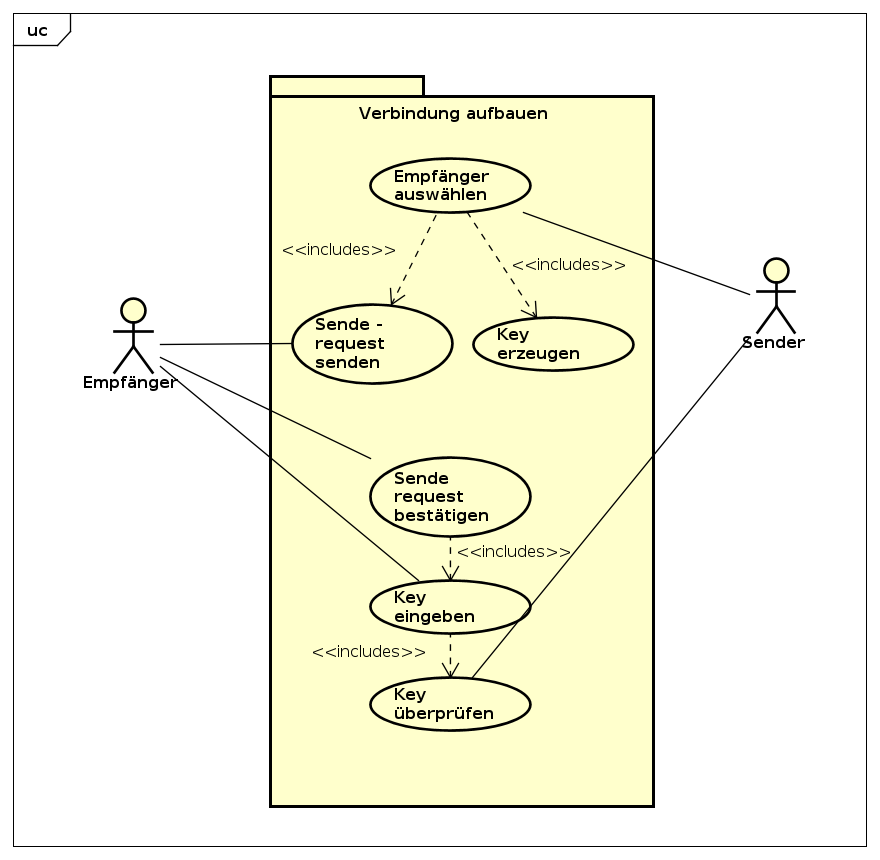
\includegraphics[width= 0.9\linewidth]{diagramms/useCase/verbindung_aufbauen.png}
	\caption{Verbindung aufbauen}
\end{figure}
Wenn der Sender nun die Datei ausgewählt hat muss er einen Empfänger auswählen. Nachdem er dies getan hat, wird ein Key erzeugt und eine Sende-Request gesendet. Der Empfänger der Datei bestätigt diese und muss danach den Key eingeben. Nach der Eingabe wird geprüft ob der Key mit dem vom Sender übereinstimmt.
\newpage
\paragraph{Daten senden}\mbox{}\\
\begin{figure}[H]
	\centering
	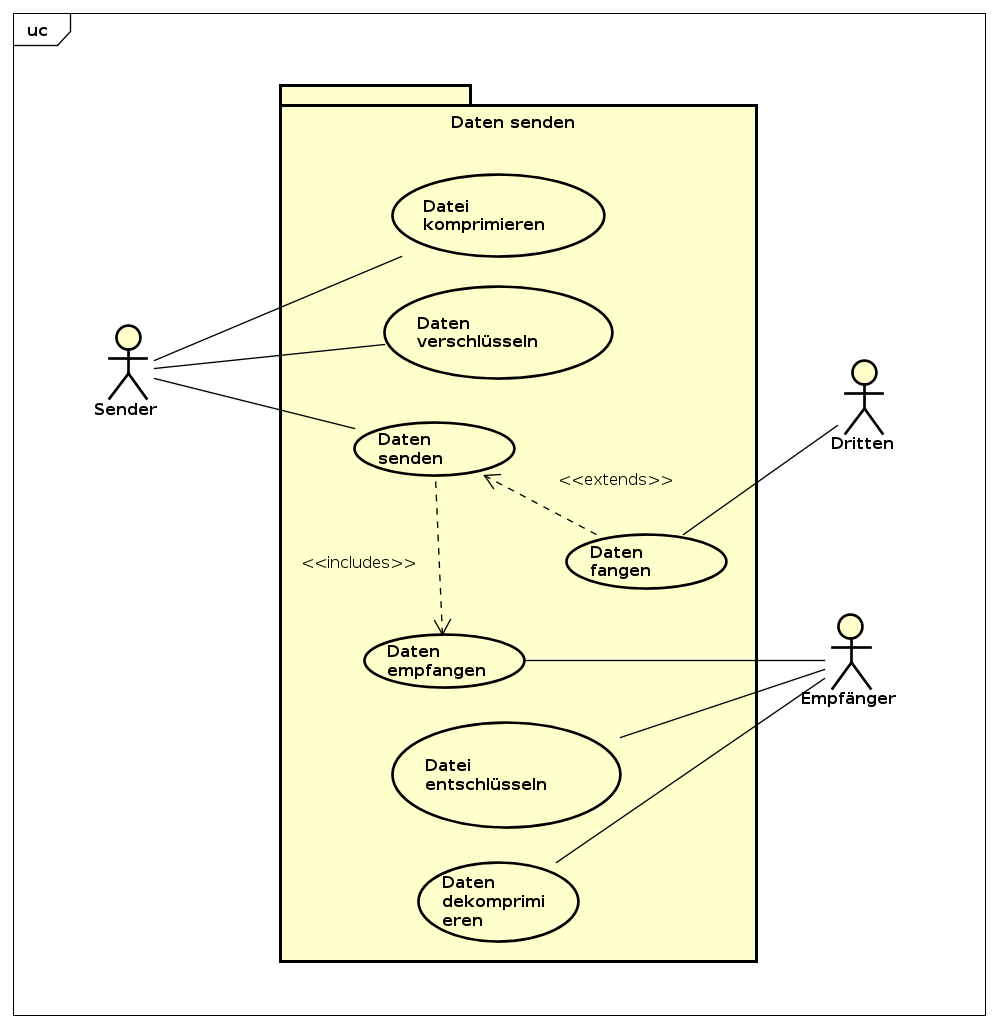
\includegraphics[width= 0.9\linewidth]{diagramms/useCase/daten_senden.png}
	\caption{Daten senden}
\end{figure}
Nachdem der Empfänger ausgewählt und der Key bestätigt wurde, wird Datei komprimiert und anschließend verschlüsselt. Wenn diese Schritte erfolgreich durchlaufen werden, wird die Datei versendet. Nun könnten die Dritten versuchen die Daten abzufangen. Falls dieser Versuch fehlschlägt oder gar nicht erst zustande erhält  der Empfänger die Datei und kann sie entschlüsseln und dekomprimieren.
\newpage
\paragraph{Datei speichern}\mbox{}\\
\begin{figure}[H]
	\centering
	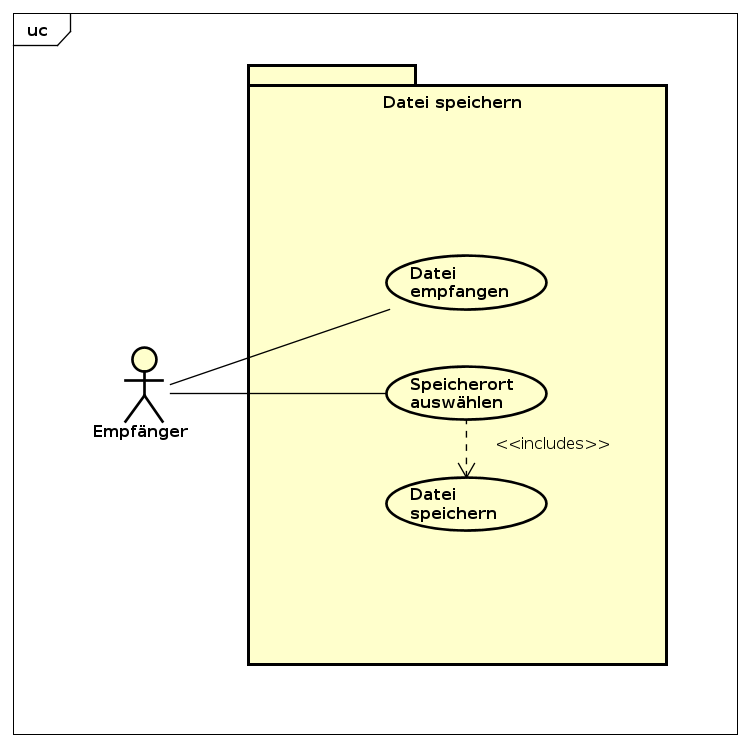
\includegraphics[width= 0.9\linewidth]{diagramms/useCase/datei_speichern.png}
	\caption{Datei speichern}
\end{figure}
Wenn der Empfänger die Datei erhält muss er einen Speicherort für sie wählen. Nachdem dieser gewählt wurde wird die Datei gespeichert. %Markus & Luca
	\newpage
	\section{Entwicklungsumgebung}
Die Entwicklungsumgebung beschreibt die Umstände der Software und Hardware, sowie der Orgware des Projektteams.
\subsection{Software}
Das Finalprodukt wird über eine Auswahl an vorinstallierten Anwendungen und integrierten Entwickleroberflächen auf den Rechnern des Projektteams geschaffen. Es werden keine weiteren Software-Lizenzen benötigt, da diese bereits gegeben sind. Dies senkt einmalige Zusatzkosten auf das Minimum. Zum Einsatz kommt hierbei die IDE Eclipse von Oracle mit dem internen WindowBuilder-Plugin.
\subsection{Hardware}
Um eine auseinandersetzungsfreie Entwicklung zu ermöglichen, werden private Notebooks und Rechensysteme für das Entwickeln des Endprodukts des Projektteams verwendet. Die Benutzung der eigenen Hardware schließt aus, dass Funktionalitäten der Software nicht auf allen System ordnungsgemäß betrieben werden können. Die Benutzung der Software setzt Betriebssysteme wie Linux-Distributionen und Windows 10, sowie die neuste Version von MacOS voraus.
\subsection{Entwicklungsschnittstellen}
Für die Datenübertragung werden gleich der späteren Anwendungen BlueTooth-Schnittstellen benutzt, da das System sonst nicht korrekt getestet und zum Laufen gebracht werden kann. Für die Orgware ist eine Internetschnittstelle von Nöten, da die meisten Zusatzmaterialien online abgesichert gespeichert sind. %Florian
	\newpage
	\section{Termine}
Es wird der Meilensteinplan mit genauen Daten und Deliverable, als auch die verschiedenen Teillieferungen vorgeführt.
\subsection{Meilensteintermine}
\begin{table}[H]
	\begin{center}
		\begin{tabularx}{\linewidth}{|X|X|X|}
			\hline
			\textbf{Meilenstein}&Deliverable&Datum\\
			\hline
			Projektstart&Alle Dokumente mit den Informationen zum Projekt&Voraussichtlich 29.03.2019\\
			\hline
			Desktop-Version&Funktionsfähige Desktop-Applikation mit allen genannten Funktionen&Voraussichtlich 26.04.2019\\
			\hline
			Smartphone-Version&Funktionsfähige Smartphone-Applikation mit allen genannten Funktionen&Voraussichtlich 11.05.2019\\
			\hline
			Produkt publizieren&Funktionsfähige Webseite mit allen genannten Funktionen. Veröffentlichtes Produkt auf Google Play Store&Voraussichtlich 20.05.2019\\
			\hline
			Projektende&Fertiges Produkt wie vereinbart&Voraussichtlich 23.05.2019\\
			\hline
		\end{tabularx}
	\end{center}
\end{table}
\subsection{Teillieferungen}
Auf die Desktop-Applikation wird besondere Priorität gesetzt weswegen sie als erstes entwickelt und übergeben werden kann. Nach dem Abschluss der ersten Teillieferung kümmert sich das Projektteam um die Entwicklung der Smartphone-Version. Wenn die Smartphone-Applikation an den Auftraggeber geliefert wird, wird die Erstellung der Webseite in Arbeit genommen. Mit der Übergabe des Webportals ist das Projekt beendet. %Markus
	\newpage
	\section{Vertragsgegenstand}
Es wird der Lieferumfang als auch die Produktbezogenen Leistungen ,welche vom Auftraggeber nach Übergabe der Produkte angefordert werden können, beschrieben.
\subsection{Lieferumfang}
Nach Abschluss des Projekts wird dem Auftraggeber eine Funktionsfähige Desktop-Applikation wie auch eine Smartphone-Version und ein Webportal übergeben. All diese Produkte enthalten, alle in dem Pflichtenheft enthaltenen, Produktfunktionen. Zu Installation für die beiden Applikationen, wird es eine Installationsdatei geben welche sich von der passenden Plattform heruntergeladen werden kann. Nach download der Datei kann diese ausgeführt werden und der Benutzer kann die Applikation erfolgreich installieren. 
\\\\
Mit der Lieferung der Produkte, werden jegliche Rechte an den Auftraggeber übergeben.
\subsection{Produktbezogene Leistungen}
Bis ein Monat nach Produktübergabe ist der Auftragnehmer verpflichtet jegliche Fehler in der Software zu beheben. Nach dieser Frist kann sich der Auftraggeber bei Bedarf wieder an den Auftragnehmer wenden und eine Fehlerbehebung anfordern. Je nach Fehlergröße muss der Auftraggeber natürlich einen entsprechenden Preis bezahlen. Ebenfalls kann man auch Patches für die Software anfordern. Der Preis wird, genau wie die Fehlerbehebung, nach dem Aufwand bezahlt. %Markus
	\newpage
	\section{Sonstiges}
Es werden die sonstigen Bedingungen welche sich auf das Produkt beziehen beschrieben. Diese können sich auf verschiedenen Aspektes beziehen und sind nicht immer in ihrer Wichtigkeit als nieder anzusehen.

\begin{indentE}\mbox{}
	\paragraph{Desktop vs. App}\mbox{}\\
	Es wird ein sehr große Priorität auf die Desktop-Version gelegt. Diese prägt sich auch darauf aus, das die App im Falle, dass die Desktop-Version droht nicht fertig zu werden, sogar gestrichen werden, solang dies dem Auftraggeber mitgeteilt wird. Falls die App-Version zustande kommt verpflichtet sich aber der Auftraggeber dem Auftragnehmer eine Prämie von 5000€ zu bezahlen.
	
	\paragraph{Webseite aufsetzen}\mbox{}\\
	Der Auftragnehmer wie in den Abgrenzungskriterien beschrieben verpflichtet sich nicht dazu die Webseite aufzusetzen, auf welche das Produkt grundsätzlich vermarktet werden soll. Deshalb muss dies entweder vom Auftraggeber selbst organisiert werden oder der Auftragnehmer anhand eines eigenen Vertrages dafür verantwortlich gemacht werden, was natürlich zu zusätzlichen Kosten führt.
	
	\paragraph{Bugfixes}\mbox{}\\
	Falls nach der ausgemachten Projekt und Nachtbetreuungszeit Fehler mit der Software oder Upgrades dieser geplant werden. Muss dies selbst organisiert werden oder man kann den Auftragnehmer durch einen neuen Vertrag dazu beauftragen.
\end{indentE}
 %Georg
	\newpage
	\section{Glossar}
Das \textbf{Backend} beschreibt die Schnittstelle zwischen einem Rechengerät und einer Software. Sie enthält die Funktionen, meist in einer Programmiersprache umgesetzt. Backend und Frontend sind zu unterscheiden.
\\
\\
\textbf{Windows 10} ist das aktuellste Betriebssystem der Microsoft Windows NT Serie. Es stellt ein System für ein Rechengerät dar.
\\
\\
\textbf{Android 8.0} oder auch 'Oreo' genannt. Ist die am häufigst genutzte Google Android Version, welche noch aktuell ist. Sie bietet ein Betriebssystem für Smartphones, jedoch nicht für Apple iPhones. Android ist meist OEM und kostenfrei.
\\
\\
\textbf{Debian 9} ist eine sehr beliebte Linux-Distribution, die noch oft im Einsatz von kleineren Firmen und Privatanwendern ist. Es ist ein kostenfreies Betriebssystem.
\\
\\
\textbf{macOS} ist das einzige Betriebssystem für Rechensysteme von Apple und wird nur für die Eigenmarken verwendet.
\\
\\
\textbf{iOS} ist das einzige Betriebssystem für Smartphones von Apple und wird ebenso nur für die Eigenmarken verwendet.
\\
\\
Mit dem \textbf{Frontend} wird die Schnittstelle zwischen der Software und dem Anwender beschrieben. Sie wird auch oft als grafische Darstellung einer Software bezeichnet.
\\
\\
Mit dem \textbf{Desktopinterface} ist das Frontend der Desktopapplikation gemeint.
\\
\\
Mit dem \textbf{Appinterface} ist das Frontend der App gemeint.
\\
\\
Der \textbf{Play Store} ist das Application-Prividing-System von Google auf dem Android-Betriebssystem.
\\
\\
Der \textbf{App Store} ist das Application-Providing-System von Apple auf dem macOS- und iOS-Betriebssystem.
\\
\\
\textbf{BlueTooth} beschreibt die Übertragungsschnittstelle, welche nur auf einem kleinen Bereich wirksam ist. Sie entspricht dem Standard IEEE 802.15.1. %Florian
\end{document}